\documentclass[twoside]{book}

% Packages required by doxygen
\usepackage{fixltx2e}
\usepackage{calc}
\usepackage{doxygen}
\usepackage[export]{adjustbox} % also loads graphicx
\usepackage{graphicx}
\usepackage[utf8]{inputenc}
\usepackage{makeidx}
\usepackage{multicol}
\usepackage{multirow}
\PassOptionsToPackage{warn}{textcomp}
\usepackage{textcomp}
\usepackage[nointegrals]{wasysym}
\usepackage[table]{xcolor}

% Font selection
\usepackage[T1]{fontenc}
\usepackage[scaled=.90]{helvet}
\usepackage{courier}
\usepackage{amssymb}
\usepackage{sectsty}
\renewcommand{\familydefault}{\sfdefault}
\allsectionsfont{%
  \fontseries{bc}\selectfont%
  \color{darkgray}%
}
\renewcommand{\DoxyLabelFont}{%
  \fontseries{bc}\selectfont%
  \color{darkgray}%
}
\newcommand{\+}{\discretionary{\mbox{\scriptsize$\hookleftarrow$}}{}{}}

% Page & text layout
\usepackage{geometry}
\geometry{%
  a4paper,%
  top=2.5cm,%
  bottom=2.5cm,%
  left=2.5cm,%
  right=2.5cm%
}
\tolerance=750
\hfuzz=15pt
\hbadness=750
\setlength{\emergencystretch}{15pt}
\setlength{\parindent}{0cm}
\setlength{\parskip}{3ex plus 2ex minus 2ex}
\makeatletter
\renewcommand{\paragraph}{%
  \@startsection{paragraph}{4}{0ex}{-1.0ex}{1.0ex}{%
    \normalfont\normalsize\bfseries\SS@parafont%
  }%
}
\renewcommand{\subparagraph}{%
  \@startsection{subparagraph}{5}{0ex}{-1.0ex}{1.0ex}{%
    \normalfont\normalsize\bfseries\SS@subparafont%
  }%
}
\makeatother

% Headers & footers
\usepackage{fancyhdr}
\pagestyle{fancyplain}
\fancyhead[LE]{\fancyplain{}{\bfseries\thepage}}
\fancyhead[CE]{\fancyplain{}{}}
\fancyhead[RE]{\fancyplain{}{\bfseries\leftmark}}
\fancyhead[LO]{\fancyplain{}{\bfseries\rightmark}}
\fancyhead[CO]{\fancyplain{}{}}
\fancyhead[RO]{\fancyplain{}{\bfseries\thepage}}
\fancyfoot[LE]{\fancyplain{}{}}
\fancyfoot[CE]{\fancyplain{}{}}
\fancyfoot[RE]{\fancyplain{}{\bfseries\scriptsize Generated by Doxygen }}
\fancyfoot[LO]{\fancyplain{}{\bfseries\scriptsize Generated by Doxygen }}
\fancyfoot[CO]{\fancyplain{}{}}
\fancyfoot[RO]{\fancyplain{}{}}
\renewcommand{\footrulewidth}{0.4pt}
\renewcommand{\chaptermark}[1]{%
  \markboth{#1}{}%
}
\renewcommand{\sectionmark}[1]{%
  \markright{\thesection\ #1}%
}

% Indices & bibliography
\usepackage{natbib}
\usepackage[titles]{tocloft}
\setcounter{tocdepth}{3}
\setcounter{secnumdepth}{5}
\makeindex

% Hyperlinks (required, but should be loaded last)
\usepackage{ifpdf}
\ifpdf
  \usepackage[pdftex,pagebackref=true]{hyperref}
\else
  \usepackage[ps2pdf,pagebackref=true]{hyperref}
\fi
\hypersetup{%
  colorlinks=true,%
  linkcolor=blue,%
  citecolor=blue,%
  unicode%
}

% Custom commands
\newcommand{\clearemptydoublepage}{%
  \newpage{\pagestyle{empty}\cleardoublepage}%
}

\usepackage{caption}
\captionsetup{labelsep=space,justification=centering,font={bf},singlelinecheck=off,skip=4pt,position=top}

%===== C O N T E N T S =====

\begin{document}

% Titlepage & ToC
\hypersetup{pageanchor=false,
             bookmarksnumbered=true,
             pdfencoding=unicode
            }
\pagenumbering{roman}
\begin{titlepage}
\vspace*{7cm}
\begin{center}%
{\Large Shell\+Project }\\
\vspace*{1cm}
{\large Generated by Doxygen 1.8.11}\\
\end{center}
\end{titlepage}
\clearemptydoublepage
\tableofcontents
\clearemptydoublepage
\pagenumbering{arabic}
\hypersetup{pageanchor=true}

%--- Begin generated contents ---
\chapter{Class Index}
\section{Class List}
Here are the classes, structs, unions and interfaces with brief descriptions\+:\begin{DoxyCompactList}
\item\contentsline{section}{\hyperlink{struct__node}{\+\_\+node} }{\pageref{struct__node}}{}
\item\contentsline{section}{\hyperlink{structnlist}{nlist} }{\pageref{structnlist}}{}
\end{DoxyCompactList}

\chapter{File Index}
\section{File List}
Here is a list of all documented files with brief descriptions\+:\begin{DoxyCompactList}
\item\contentsline{section}{header/\hyperlink{cmd_8h}{cmd.\+h} \\*Fichier contenant les fonctions utiles aux commandes shell }{\pageref{cmd_8h}}{}
\item\contentsline{section}{header/\hyperlink{hash_8h}{hash.\+h} \\*Fichier contenant les fonctions utiles à un Hash\+Map. Code source venant de Section 6.\+6 of The C Programming Language }{\pageref{hash_8h}}{}
\item\contentsline{section}{header/\hyperlink{helper_8h}{helper.\+h} \\*Helper header }{\pageref{helper_8h}}{}
\item\contentsline{section}{header/\hyperlink{log_8h}{log.\+h} \\*Log header }{\pageref{log_8h}}{}
\item\contentsline{section}{header/\hyperlink{shell_8h}{shell.\+h} \\*Header principal }{\pageref{shell_8h}}{}
\item\contentsline{section}{header/\hyperlink{tree_8h}{tree.\+h} \\*Librairie permettant l\textquotesingle{}utilisation d\textquotesingle{}un tree }{\pageref{tree_8h}}{}
\item\contentsline{section}{header/\hyperlink{typedef_8h}{typedef.\+h} \\*Définition des variables, enum, struct }{\pageref{typedef_8h}}{}
\item\contentsline{section}{src/\hyperlink{hash_8c}{hash.\+c} \\*Fichier contenant les fonctions utiles à un Hash\+Map. Code source venant de Section 6.\+6 of The C Programming Language }{\pageref{hash_8c}}{}
\item\contentsline{section}{src/\hyperlink{helper_8c}{helper.\+c} \\*Fichier contenant les fonctions d\textquotesingle{}helper }{\pageref{helper_8c}}{}
\item\contentsline{section}{src/\hyperlink{log_8c}{log.\+c} \\*Interaction fichier log }{\pageref{log_8c}}{}
\end{DoxyCompactList}

\chapter{Class Documentation}
\hypertarget{struct__node}{}\section{\+\_\+node Struct Reference}
\label{struct__node}\index{\+\_\+node@{\+\_\+node}}


Collaboration diagram for \+\_\+node\+:\nopagebreak
\begin{figure}[H]
\begin{center}
\leavevmode
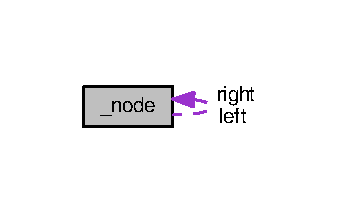
\includegraphics[width=163pt]{struct__node__coll__graph}
\end{center}
\end{figure}
\subsection*{Public Attributes}
\begin{DoxyCompactItemize}
\item 
char $\ast$ {\bfseries value}\hypertarget{struct__node_a10fea5606d2e5925640c53baef7c10d9}{}\label{struct__node_a10fea5606d2e5925640c53baef7c10d9}

\item 
struct \hyperlink{struct__node}{\+\_\+node} $\ast$ {\bfseries left}\hypertarget{struct__node_ac655c71579c94517b53fbb59d99829bf}{}\label{struct__node_ac655c71579c94517b53fbb59d99829bf}

\item 
struct \hyperlink{struct__node}{\+\_\+node} $\ast$ {\bfseries right}\hypertarget{struct__node_a0958469df50896d9eb5dbaac2e7db7bb}{}\label{struct__node_a0958469df50896d9eb5dbaac2e7db7bb}

\end{DoxyCompactItemize}


The documentation for this struct was generated from the following file\+:\begin{DoxyCompactItemize}
\item 
header/\hyperlink{typedef_8h}{typedef.\+h}\end{DoxyCompactItemize}

\hypertarget{structnlist}{}\section{nlist Struct Reference}
\label{structnlist}\index{nlist@{nlist}}


Collaboration diagram for nlist\+:\nopagebreak
\begin{figure}[H]
\begin{center}
\leavevmode
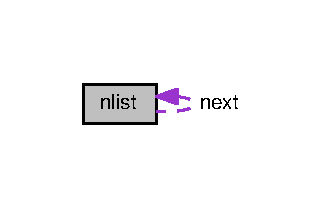
\includegraphics[width=155pt]{structnlist__coll__graph}
\end{center}
\end{figure}
\subsection*{Public Attributes}
\begin{DoxyCompactItemize}
\item 
struct \hyperlink{structnlist}{nlist} $\ast$ {\bfseries next}\hypertarget{structnlist_a6e5fbb2f12a2799e60611dbda92c6f38}{}\label{structnlist_a6e5fbb2f12a2799e60611dbda92c6f38}

\item 
char $\ast$ {\bfseries name}\hypertarget{structnlist_adae5489b500836e59f19fad605a63b07}{}\label{structnlist_adae5489b500836e59f19fad605a63b07}

\item 
char $\ast$ {\bfseries defn}\hypertarget{structnlist_a1405526a048e968f43d1b8495d5143ca}{}\label{structnlist_a1405526a048e968f43d1b8495d5143ca}

\end{DoxyCompactItemize}


The documentation for this struct was generated from the following file\+:\begin{DoxyCompactItemize}
\item 
header/\hyperlink{typedef_8h}{typedef.\+h}\end{DoxyCompactItemize}

\chapter{File Documentation}
\hypertarget{cmd_8h}{}\section{header/cmd.h File Reference}
\label{cmd_8h}\index{header/cmd.\+h@{header/cmd.\+h}}


Fichier contenant les fonctions utiles aux commandes shell.  


{\ttfamily \#include \char`\"{}typedef.\+h\char`\"{}}\\*
{\ttfamily \#include \char`\"{}helper.\+h\char`\"{}}\\*
Include dependency graph for cmd.\+h\+:\nopagebreak
\begin{figure}[H]
\begin{center}
\leavevmode
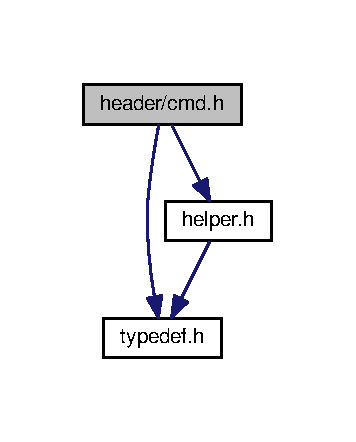
\includegraphics[width=171pt]{cmd_8h__incl}
\end{center}
\end{figure}
\subsection*{Functions}
\begin{DoxyCompactItemize}
\item 
void \hyperlink{cmd_8h_a56a8e2df9cc1b51768282c3c25874038}{run\+Help} ()
\begin{DoxyCompactList}\small\item\em Fonction permettant la lecture d\textquotesingle{}un help. \end{DoxyCompactList}\item 
int \hyperlink{cmd_8h_a9ba7160033643930ae009566f7249495}{execute} (char $\ast$$\ast$args)
\begin{DoxyCompactList}\small\item\em Fonction permettant de rediriger les commandes vers les fonctions d\textquotesingle{}executions corespondantes. \end{DoxyCompactList}\item 
void \hyperlink{cmd_8h_ad7f750d44fbfd1fe9bb336972c061301}{print\+Dir} ()
\begin{DoxyCompactList}\small\item\em Fonction permettant d\textquotesingle{}afficher le dossier courant lors de l\textquotesingle{}attente d\textquotesingle{}une saisie dans l\textquotesingle{}entrée standard. \end{DoxyCompactList}\item 
int \hyperlink{cmd_8h_a22c46228fb3fc251965314bc14b0962e}{run\+Command} (char $\ast$$\ast$args)
\begin{DoxyCompactList}\small\item\em Fonction permettant l\textquotesingle{}execution via un fork et execvp des commandes simples du shell. \end{DoxyCompactList}\item 
int \hyperlink{cmd_8h_aa360d03ba8c90797bd1466b790c10fe6}{run\+Cd} (char $\ast$$\ast$args)
\begin{DoxyCompactList}\small\item\em Fonction permettant l\textquotesingle{}execution de la fonction build in cd. \end{DoxyCompactList}\item 
\hyperlink{typedef_8h_a1062901a7428fdd9c7f180f5e01ea056}{bool} \hyperlink{cmd_8h_ab591853ba45fab61ee9bb76304f72a61}{run\+Echo} (char $\ast$str)
\begin{DoxyCompactList}\small\item\em Fonction permettant l\textquotesingle{}exectuion de la fonction build in echo. \end{DoxyCompactList}\end{DoxyCompactItemize}


\subsection{Detailed Description}
Fichier contenant les fonctions utiles aux commandes shell. 

\begin{DoxyAuthor}{Author}
lfreyss 
\end{DoxyAuthor}
\begin{DoxyVersion}{Version}
0.\+1 
\end{DoxyVersion}
\begin{DoxyDate}{Date}
20180301
\end{DoxyDate}
Fichier contenant les fonctionnalités cmd . 

\subsection{Function Documentation}
\index{cmd.\+h@{cmd.\+h}!execute@{execute}}
\index{execute@{execute}!cmd.\+h@{cmd.\+h}}
\subsubsection[{\texorpdfstring{execute(char $\ast$$\ast$args)}{execute(char **args)}}]{\setlength{\rightskip}{0pt plus 5cm}int execute (
\begin{DoxyParamCaption}
\item[{char $\ast$$\ast$}]{args}
\end{DoxyParamCaption}
)}\hypertarget{cmd_8h_a9ba7160033643930ae009566f7249495}{}\label{cmd_8h_a9ba7160033643930ae009566f7249495}


Fonction permettant de rediriger les commandes vers les fonctions d\textquotesingle{}executions corespondantes. 

\begin{DoxyAuthor}{Author}
vlambs 
\end{DoxyAuthor}

\begin{DoxyParams}{Parameters}
{\em tableau} & de string contenant la commande a éxécuter et ses arguments/options \\
\hline
\end{DoxyParams}
\begin{DoxyReturn}{Returns}
void 
\end{DoxyReturn}
\index{cmd.\+h@{cmd.\+h}!print\+Dir@{print\+Dir}}
\index{print\+Dir@{print\+Dir}!cmd.\+h@{cmd.\+h}}
\subsubsection[{\texorpdfstring{print\+Dir()}{printDir()}}]{\setlength{\rightskip}{0pt plus 5cm}void print\+Dir (
\begin{DoxyParamCaption}
{}
\end{DoxyParamCaption}
)}\hypertarget{cmd_8h_ad7f750d44fbfd1fe9bb336972c061301}{}\label{cmd_8h_ad7f750d44fbfd1fe9bb336972c061301}


Fonction permettant d\textquotesingle{}afficher le dossier courant lors de l\textquotesingle{}attente d\textquotesingle{}une saisie dans l\textquotesingle{}entrée standard. 

\begin{DoxyAuthor}{Author}
lfreyss 
\end{DoxyAuthor}

\begin{DoxyParams}{Parameters}
{\em void} & \\
\hline
\end{DoxyParams}
\begin{DoxyReturn}{Returns}
void 
\end{DoxyReturn}
\index{cmd.\+h@{cmd.\+h}!run\+Cd@{run\+Cd}}
\index{run\+Cd@{run\+Cd}!cmd.\+h@{cmd.\+h}}
\subsubsection[{\texorpdfstring{run\+Cd(char $\ast$$\ast$args)}{runCd(char **args)}}]{\setlength{\rightskip}{0pt plus 5cm}int run\+Cd (
\begin{DoxyParamCaption}
\item[{char $\ast$$\ast$}]{args}
\end{DoxyParamCaption}
)}\hypertarget{cmd_8h_aa360d03ba8c90797bd1466b790c10fe6}{}\label{cmd_8h_aa360d03ba8c90797bd1466b790c10fe6}


Fonction permettant l\textquotesingle{}execution de la fonction build in cd. 

\begin{DoxyAuthor}{Author}
vlambs 
\end{DoxyAuthor}

\begin{DoxyParams}{Parameters}
{\em tableau} & de string contenant la commande a éxécuter et ses arguments/options \\
\hline
\end{DoxyParams}
\begin{DoxyReturn}{Returns}
Succès de la commande ou non 
\end{DoxyReturn}
\index{cmd.\+h@{cmd.\+h}!run\+Command@{run\+Command}}
\index{run\+Command@{run\+Command}!cmd.\+h@{cmd.\+h}}
\subsubsection[{\texorpdfstring{run\+Command(char $\ast$$\ast$args)}{runCommand(char **args)}}]{\setlength{\rightskip}{0pt plus 5cm}int run\+Command (
\begin{DoxyParamCaption}
\item[{char $\ast$$\ast$}]{args}
\end{DoxyParamCaption}
)}\hypertarget{cmd_8h_a22c46228fb3fc251965314bc14b0962e}{}\label{cmd_8h_a22c46228fb3fc251965314bc14b0962e}


Fonction permettant l\textquotesingle{}execution via un fork et execvp des commandes simples du shell. 

\begin{DoxyAuthor}{Author}
vlambs/lfreyss 
\end{DoxyAuthor}

\begin{DoxyParams}{Parameters}
{\em tableau} & de string contenant la commande a éxécuter et ses arguments/options \\
\hline
\end{DoxyParams}
\begin{DoxyReturn}{Returns}
Succès de la commande ou non 
\end{DoxyReturn}
\index{cmd.\+h@{cmd.\+h}!run\+Echo@{run\+Echo}}
\index{run\+Echo@{run\+Echo}!cmd.\+h@{cmd.\+h}}
\subsubsection[{\texorpdfstring{run\+Echo(char $\ast$str)}{runEcho(char *str)}}]{\setlength{\rightskip}{0pt plus 5cm}{\bf bool} run\+Echo (
\begin{DoxyParamCaption}
\item[{char $\ast$}]{str}
\end{DoxyParamCaption}
)}\hypertarget{cmd_8h_ab591853ba45fab61ee9bb76304f72a61}{}\label{cmd_8h_ab591853ba45fab61ee9bb76304f72a61}


Fonction permettant l\textquotesingle{}exectuion de la fonction build in echo. 

\begin{DoxyAuthor}{Author}
lfreyss 
\end{DoxyAuthor}

\begin{DoxyParams}{Parameters}
{\em tableau} & de string contenant la commande a éxécuter et ses arguments/options \\
\hline
\end{DoxyParams}
\begin{DoxyReturn}{Returns}
Succès de la commande ou non 
\end{DoxyReturn}
\index{cmd.\+h@{cmd.\+h}!run\+Help@{run\+Help}}
\index{run\+Help@{run\+Help}!cmd.\+h@{cmd.\+h}}
\subsubsection[{\texorpdfstring{run\+Help()}{runHelp()}}]{\setlength{\rightskip}{0pt plus 5cm}void run\+Help (
\begin{DoxyParamCaption}
{}
\end{DoxyParamCaption}
)}\hypertarget{cmd_8h_a56a8e2df9cc1b51768282c3c25874038}{}\label{cmd_8h_a56a8e2df9cc1b51768282c3c25874038}


Fonction permettant la lecture d\textquotesingle{}un help. 

\begin{DoxyAuthor}{Author}
vlambs 
\end{DoxyAuthor}

\begin{DoxyParams}{Parameters}
{\em } & \\
\hline
\end{DoxyParams}

\hypertarget{hash_8h}{}\section{header/hash.h File Reference}
\label{hash_8h}\index{header/hash.\+h@{header/hash.\+h}}


Fichier contenant les fonctions utiles à un Hash\+Map. Code source venant de Section 6.\+6 of The C Programming Language.  


{\ttfamily \#include \char`\"{}typedef.\+h\char`\"{}}\\*
Include dependency graph for hash.\+h\+:\nopagebreak
\begin{figure}[H]
\begin{center}
\leavevmode
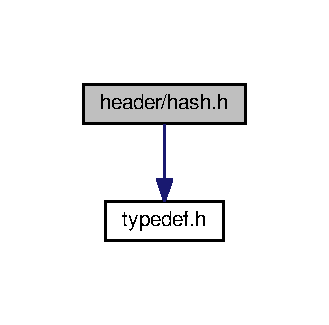
\includegraphics[width=158pt]{hash_8h__incl}
\end{center}
\end{figure}
\subsection*{Functions}
\begin{DoxyCompactItemize}
\item 
unsigned {\bfseries hash} (char $\ast$s)\hypertarget{hash_8h_a998ad9aa6cfe8a43b60cdc806667bdb2}{}\label{hash_8h_a998ad9aa6cfe8a43b60cdc806667bdb2}

\item 
struct \hyperlink{structnlist}{nlist} $\ast$ \hyperlink{hash_8h_aade07f4a46f6b9dc676fb0bca7249f5b}{lookup} (char $\ast$s)
\begin{DoxyCompactList}\small\item\em Fonction permettant de parcourir la Hash\+Map et de trouver l\textquotesingle{}élement voulu. \end{DoxyCompactList}\item 
struct \hyperlink{structnlist}{nlist} $\ast$ \hyperlink{hash_8h_af3277df8a8588aab5b389118781e199e}{install} (char $\ast$name, char $\ast$defn)
\begin{DoxyCompactList}\small\item\em Fonction permettant de rajouter un élément à la Hash\+Map. \end{DoxyCompactList}\end{DoxyCompactItemize}


\subsection{Detailed Description}
Fichier contenant les fonctions utiles à un Hash\+Map. Code source venant de Section 6.\+6 of The C Programming Language. 

\begin{DoxyAuthor}{Author}
lfreyss 
\end{DoxyAuthor}
\begin{DoxyVersion}{Version}
0.\+1 
\end{DoxyVersion}
\begin{DoxyDate}{Date}
20180308
\end{DoxyDate}
Fichier contenant les fonctionnalités H\+A\+SH . 

\subsection{Function Documentation}
\index{hash.\+h@{hash.\+h}!install@{install}}
\index{install@{install}!hash.\+h@{hash.\+h}}
\subsubsection[{\texorpdfstring{install(char $\ast$name, char $\ast$defn)}{install(char *name, char *defn)}}]{\setlength{\rightskip}{0pt plus 5cm}{\bf bool} {\bf nlist} $\ast$ install (
\begin{DoxyParamCaption}
\item[{char $\ast$}]{name, }
\item[{char $\ast$}]{defn}
\end{DoxyParamCaption}
)}\hypertarget{hash_8h_af3277df8a8588aab5b389118781e199e}{}\label{hash_8h_af3277df8a8588aab5b389118781e199e}


Fonction permettant de rajouter un élément à la Hash\+Map. 

\begin{DoxyAuthor}{Author}
lfreyss 
\end{DoxyAuthor}

\begin{DoxyParams}{Parameters}
{\em name} & -\/$>$ nom du hashmap; defn -\/$>$ valeur du hashmap \\
\hline
\end{DoxyParams}
\begin{DoxyReturn}{Returns}
nlist que l\textquotesingle{}on vient de rajouter 
\end{DoxyReturn}
\index{hash.\+h@{hash.\+h}!lookup@{lookup}}
\index{lookup@{lookup}!hash.\+h@{hash.\+h}}
\subsubsection[{\texorpdfstring{lookup(char $\ast$s)}{lookup(char *s)}}]{\setlength{\rightskip}{0pt plus 5cm}struct {\bf nlist} $\ast$ lookup (
\begin{DoxyParamCaption}
\item[{char $\ast$}]{s}
\end{DoxyParamCaption}
)}\hypertarget{hash_8h_aade07f4a46f6b9dc676fb0bca7249f5b}{}\label{hash_8h_aade07f4a46f6b9dc676fb0bca7249f5b}


Fonction permettant de parcourir la Hash\+Map et de trouver l\textquotesingle{}élement voulu. 

\begin{DoxyAuthor}{Author}
lfreyss 
\end{DoxyAuthor}

\begin{DoxyParams}{Parameters}
{\em chaine} & de caractère que l\textquotesingle{}on recherche \\
\hline
\end{DoxyParams}
\begin{DoxyReturn}{Returns}
Struct nlist recherchée ou null si non trouvée 
\end{DoxyReturn}

\hypertarget{helper_8h}{}\section{header/helper.h File Reference}
\label{helper_8h}\index{header/helper.\+h@{header/helper.\+h}}


helper header.  


{\ttfamily \#include \char`\"{}typedef.\+h\char`\"{}}\\*
Include dependency graph for helper.\+h\+:\nopagebreak
\begin{figure}[H]
\begin{center}
\leavevmode
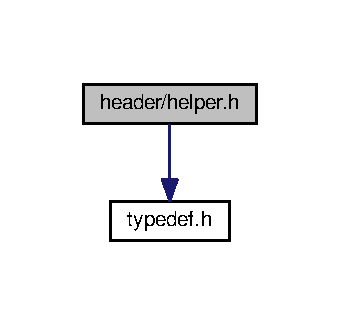
\includegraphics[width=163pt]{helper_8h__incl}
\end{center}
\end{figure}
This graph shows which files directly or indirectly include this file\+:\nopagebreak
\begin{figure}[H]
\begin{center}
\leavevmode
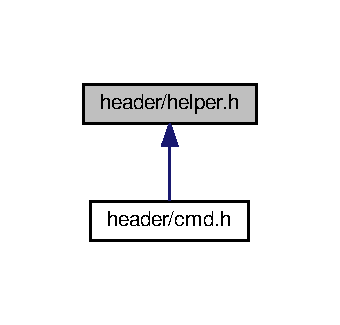
\includegraphics[width=163pt]{helper_8h__dep__incl}
\end{center}
\end{figure}
\subsection*{Functions}
\begin{DoxyCompactItemize}
\item 
char $\ast$ \hyperlink{helper_8h_aac413c02d8c475ff10cfd02904180d89}{readline} (void)
\begin{DoxyCompactList}\small\item\em Fonction permettant de lire la saisie de l\textquotesingle{}entrée standard. \end{DoxyCompactList}\item 
int \hyperlink{helper_8h_a1e941fcaa0b19e24f436561f13fff047}{parse\+Space} (char $\ast$str, char $\ast$parsed\mbox{[}$\,$\mbox{]})
\begin{DoxyCompactList}\small\item\em Fonction permettant de séparer une chaine de caractère par des espaces. \end{DoxyCompactList}\item 
int \hyperlink{helper_8h_a1db78452432b56ef399a0b054b62a638}{parse\+String} (char $\ast$str, char $\ast$parsed\mbox{[}$\,$\mbox{]}, char $\ast$sep)
\begin{DoxyCompactList}\small\item\em Fonction permettant de séparer une chaine de caractère par un caractère pré-\/définie. \end{DoxyCompactList}\item 
void \hyperlink{helper_8h_a1d9ff13ca6fbfeed019ff8459a2d7b27}{ltrim} (char $\ast$str)
\begin{DoxyCompactList}\small\item\em Fonction permettant de supprimer les espaces, les tabulations et sauts de ligne en début de string. \end{DoxyCompactList}\item 
void \hyperlink{helper_8h_a36c31afc53e5a1e87177eff988d6d17e}{rtrim} (char $\ast$str)
\begin{DoxyCompactList}\small\item\em Fonction permettant de supprimer les espaces, les tabulations et sauts de ligne en fin de string. \end{DoxyCompactList}\item 
void \hyperlink{helper_8h_a67a5c19d5a2782a49836a0b9190b88f8}{trim} (char str\mbox{[}$\,$\mbox{]})
\begin{DoxyCompactList}\small\item\em Fonction permettant d\textquotesingle{}appeler le rtrim et ltrim en un seul appel. \end{DoxyCompactList}\item 
void \hyperlink{helper_8h_a18c4769c27205c182ebca5ff7499c1ab}{add\+Char} (char c, char $\ast$string\+To\+Add)
\begin{DoxyCompactList}\small\item\em Concatène un caractère à une chaine de caractère. \end{DoxyCompactList}\item 
int \hyperlink{helper_8h_a6dc328bf1c07bf8d8c87aab9ab66658f}{parse\+Control\+Operator} (char $\ast$str, char $\ast$$\ast$parsed)
\begin{DoxyCompactList}\small\item\em Fonction permettant de découper une string par les opérateurs de control, à savoir \&\& et $\vert$$\vert$. \end{DoxyCompactList}\item 
int \hyperlink{helper_8h_a983ac2428db05783a35c1341febb9d37}{parse\+Redirection\+Flux} (char $\ast$str, char $\ast$$\ast$parsed)
\begin{DoxyCompactList}\small\item\em Fonction permettant de découper une string par les opérateurs de redirection de flux, à savoir $\vert$,\&,$<$,$>$,$<$$<$,$>$$>$ \end{DoxyCompactList}\item 
char $\ast$$\ast$ \hyperlink{helper_8h_a8db428717c03dd88f89e0995ac5aa3bb}{create\+Calloc\+Tab} (int x, int y)
\begin{DoxyCompactList}\small\item\em Fonction permettant de créer un tableau de chaine de caractère. \end{DoxyCompactList}\item 
void \hyperlink{helper_8h_a00eacdb7422e4261253801a228a102a0}{copy\+Content\+File} (char $\ast$writefilename, char $\ast$readfilename, \hyperlink{typedef_8h_a1062901a7428fdd9c7f180f5e01ea056}{bool} overide)
\begin{DoxyCompactList}\small\item\em Fonction permettant la copie du contenu d\textquotesingle{}un fichier vers un autre. \end{DoxyCompactList}\item 
\hyperlink{typedef_8h_a1062901a7428fdd9c7f180f5e01ea056}{bool} \hyperlink{helper_8h_a9b39605351f88642b3f802a77a607185}{file\+Is\+Empty} ()
\begin{DoxyCompactList}\small\item\em Fonction permettant de check si un fichier est vide ou non. \end{DoxyCompactList}\item 
void \hyperlink{helper_8h_aaebc21a8340b94ee50729f1d95a3b389}{display\+Output} (char $\ast$filename)
\begin{DoxyCompactList}\small\item\em Fonction permettant de afficher le contenu d\textquotesingle{}un fichier sur la sortie standard. \end{DoxyCompactList}\item 
void \hyperlink{helper_8h_a91810b2c3cb895cb752b64be77c8c4a1}{add\+Content\+To\+File} (char $\ast$str)
\begin{DoxyCompactList}\small\item\em Fonction permettant de rajouter du contenu à un fichier. \end{DoxyCompactList}\end{DoxyCompactItemize}


\subsection{Detailed Description}
helper header. 

\begin{DoxyAuthor}{Author}
lfreyss 
\end{DoxyAuthor}
\begin{DoxyVersion}{Version}
0.\+1 
\end{DoxyVersion}
\begin{DoxyDate}{Date}
20180207
\end{DoxyDate}
Header principal. 

\subsection{Function Documentation}
\index{helper.\+h@{helper.\+h}!add\+Char@{add\+Char}}
\index{add\+Char@{add\+Char}!helper.\+h@{helper.\+h}}
\subsubsection[{\texorpdfstring{add\+Char(char c, char $\ast$string\+To\+Add)}{addChar(char c, char *stringToAdd)}}]{\setlength{\rightskip}{0pt plus 5cm}void add\+Char (
\begin{DoxyParamCaption}
\item[{char}]{c, }
\item[{char $\ast$}]{string\+To\+Add}
\end{DoxyParamCaption}
)}\hypertarget{helper_8h_a18c4769c27205c182ebca5ff7499c1ab}{}\label{helper_8h_a18c4769c27205c182ebca5ff7499c1ab}


Concatène un caractère à une chaine de caractère. 

\begin{DoxyAuthor}{Author}
lfreyss 
\end{DoxyAuthor}

\begin{DoxyParams}{Parameters}
{\em Caractère} & à concatèner, chaine de caractère à concatèner \\
\hline
\end{DoxyParams}
\begin{DoxyReturn}{Returns}

\end{DoxyReturn}
\index{helper.\+h@{helper.\+h}!add\+Content\+To\+File@{add\+Content\+To\+File}}
\index{add\+Content\+To\+File@{add\+Content\+To\+File}!helper.\+h@{helper.\+h}}
\subsubsection[{\texorpdfstring{add\+Content\+To\+File(char $\ast$str)}{addContentToFile(char *str)}}]{\setlength{\rightskip}{0pt plus 5cm}void add\+Content\+To\+File (
\begin{DoxyParamCaption}
\item[{char $\ast$}]{str}
\end{DoxyParamCaption}
)}\hypertarget{helper_8h_a91810b2c3cb895cb752b64be77c8c4a1}{}\label{helper_8h_a91810b2c3cb895cb752b64be77c8c4a1}


Fonction permettant de rajouter du contenu à un fichier. 

\begin{DoxyAuthor}{Author}
lfreyss 
\end{DoxyAuthor}

\begin{DoxyParams}{Parameters}
{\em String} & à ajouter au contenu du fichier \\
\hline
\end{DoxyParams}
\begin{DoxyReturn}{Returns}

\end{DoxyReturn}
\index{helper.\+h@{helper.\+h}!copy\+Content\+File@{copy\+Content\+File}}
\index{copy\+Content\+File@{copy\+Content\+File}!helper.\+h@{helper.\+h}}
\subsubsection[{\texorpdfstring{copy\+Content\+File(char $\ast$writefilename, char $\ast$readfilename, bool overide)}{copyContentFile(char *writefilename, char *readfilename, bool overide)}}]{\setlength{\rightskip}{0pt plus 5cm}void copy\+Content\+File (
\begin{DoxyParamCaption}
\item[{char $\ast$}]{writefilename, }
\item[{char $\ast$}]{readfilename, }
\item[{{\bf bool}}]{overide}
\end{DoxyParamCaption}
)}\hypertarget{helper_8h_a00eacdb7422e4261253801a228a102a0}{}\label{helper_8h_a00eacdb7422e4261253801a228a102a0}


Fonction permettant la copie du contenu d\textquotesingle{}un fichier vers un autre. 

\begin{DoxyAuthor}{Author}
lfreyss 
\end{DoxyAuthor}

\begin{DoxyParams}{Parameters}
{\em writefilename} & -\/$>$ fichier de destination, readfilename -\/$>$ fichier source, overide -\/$>$ ajouter au contenu ou le remplacer \\
\hline
\end{DoxyParams}
\begin{DoxyReturn}{Returns}

\end{DoxyReturn}
\index{helper.\+h@{helper.\+h}!create\+Calloc\+Tab@{create\+Calloc\+Tab}}
\index{create\+Calloc\+Tab@{create\+Calloc\+Tab}!helper.\+h@{helper.\+h}}
\subsubsection[{\texorpdfstring{create\+Calloc\+Tab(int x, int y)}{createCallocTab(int x, int y)}}]{\setlength{\rightskip}{0pt plus 5cm}char $\ast$$\ast$ create\+Calloc\+Tab (
\begin{DoxyParamCaption}
\item[{int}]{x, }
\item[{int}]{y}
\end{DoxyParamCaption}
)}\hypertarget{helper_8h_a8db428717c03dd88f89e0995ac5aa3bb}{}\label{helper_8h_a8db428717c03dd88f89e0995ac5aa3bb}


Fonction permettant de créer un tableau de chaine de caractère. 

\begin{DoxyAuthor}{Author}
lfreyss 
\end{DoxyAuthor}

\begin{DoxyParams}{Parameters}
{\em x} & -\/$>$ nombre de chaine de caractère, y -\/$>$ nombre de caractère dans une chaine de caractère \\
\hline
\end{DoxyParams}
\begin{DoxyReturn}{Returns}
Le tableau de chaine de caractère 
\end{DoxyReturn}
\index{helper.\+h@{helper.\+h}!display\+Output@{display\+Output}}
\index{display\+Output@{display\+Output}!helper.\+h@{helper.\+h}}
\subsubsection[{\texorpdfstring{display\+Output(char $\ast$filename)}{displayOutput(char *filename)}}]{\setlength{\rightskip}{0pt plus 5cm}void display\+Output (
\begin{DoxyParamCaption}
\item[{char $\ast$}]{filename}
\end{DoxyParamCaption}
)}\hypertarget{helper_8h_aaebc21a8340b94ee50729f1d95a3b389}{}\label{helper_8h_aaebc21a8340b94ee50729f1d95a3b389}


Fonction permettant de afficher le contenu d\textquotesingle{}un fichier sur la sortie standard. 

\begin{DoxyAuthor}{Author}
lfreyss 
\end{DoxyAuthor}

\begin{DoxyParams}{Parameters}
{\em Nom} & du fichier \\
\hline
\end{DoxyParams}
\begin{DoxyReturn}{Returns}

\end{DoxyReturn}
\index{helper.\+h@{helper.\+h}!file\+Is\+Empty@{file\+Is\+Empty}}
\index{file\+Is\+Empty@{file\+Is\+Empty}!helper.\+h@{helper.\+h}}
\subsubsection[{\texorpdfstring{file\+Is\+Empty()}{fileIsEmpty()}}]{\setlength{\rightskip}{0pt plus 5cm}{\bf bool} file\+Is\+Empty (
\begin{DoxyParamCaption}
{}
\end{DoxyParamCaption}
)}\hypertarget{helper_8h_a9b39605351f88642b3f802a77a607185}{}\label{helper_8h_a9b39605351f88642b3f802a77a607185}


Fonction permettant de check si un fichier est vide ou non. 

\begin{DoxyAuthor}{Author}
lfreyss 
\end{DoxyAuthor}

\begin{DoxyParams}{Parameters}
{\em } & \\
\hline
\end{DoxyParams}
\index{helper.\+h@{helper.\+h}!ltrim@{ltrim}}
\index{ltrim@{ltrim}!helper.\+h@{helper.\+h}}
\subsubsection[{\texorpdfstring{ltrim(char $\ast$str)}{ltrim(char *str)}}]{\setlength{\rightskip}{0pt plus 5cm}void ltrim (
\begin{DoxyParamCaption}
\item[{char $\ast$}]{str}
\end{DoxyParamCaption}
)}\hypertarget{helper_8h_a1d9ff13ca6fbfeed019ff8459a2d7b27}{}\label{helper_8h_a1d9ff13ca6fbfeed019ff8459a2d7b27}


Fonction permettant de supprimer les espaces, les tabulations et sauts de ligne en début de string. 

\begin{DoxyAuthor}{Author}
lfreyss 
\end{DoxyAuthor}

\begin{DoxyParams}{Parameters}
{\em String} & à examiner \\
\hline
\end{DoxyParams}
\begin{DoxyReturn}{Returns}

\end{DoxyReturn}
\index{helper.\+h@{helper.\+h}!parse\+Control\+Operator@{parse\+Control\+Operator}}
\index{parse\+Control\+Operator@{parse\+Control\+Operator}!helper.\+h@{helper.\+h}}
\subsubsection[{\texorpdfstring{parse\+Control\+Operator(char $\ast$str, char $\ast$$\ast$parsed)}{parseControlOperator(char *str, char **parsed)}}]{\setlength{\rightskip}{0pt plus 5cm}int parse\+Control\+Operator (
\begin{DoxyParamCaption}
\item[{char $\ast$}]{str, }
\item[{char $\ast$$\ast$}]{parsed}
\end{DoxyParamCaption}
)}\hypertarget{helper_8h_a6dc328bf1c07bf8d8c87aab9ab66658f}{}\label{helper_8h_a6dc328bf1c07bf8d8c87aab9ab66658f}


Fonction permettant de découper une string par les opérateurs de control, à savoir \&\& et $\vert$$\vert$. 

\begin{DoxyAuthor}{Author}
lfreyss 
\end{DoxyAuthor}

\begin{DoxyParams}{Parameters}
{\em String} & a découper, tab de string contenant la chaine de caractère découpé \\
\hline
\end{DoxyParams}
\begin{DoxyReturn}{Returns}
nombre de string dans le tableau 
\end{DoxyReturn}
\index{helper.\+h@{helper.\+h}!parse\+Redirection\+Flux@{parse\+Redirection\+Flux}}
\index{parse\+Redirection\+Flux@{parse\+Redirection\+Flux}!helper.\+h@{helper.\+h}}
\subsubsection[{\texorpdfstring{parse\+Redirection\+Flux(char $\ast$str, char $\ast$$\ast$parsed)}{parseRedirectionFlux(char *str, char **parsed)}}]{\setlength{\rightskip}{0pt plus 5cm}int parse\+Redirection\+Flux (
\begin{DoxyParamCaption}
\item[{char $\ast$}]{str, }
\item[{char $\ast$$\ast$}]{parsed}
\end{DoxyParamCaption}
)}\hypertarget{helper_8h_a983ac2428db05783a35c1341febb9d37}{}\label{helper_8h_a983ac2428db05783a35c1341febb9d37}


Fonction permettant de découper une string par les opérateurs de redirection de flux, à savoir $\vert$,\&,$<$,$>$,$<$$<$,$>$$>$ 

\begin{DoxyAuthor}{Author}
lfreyss 
\end{DoxyAuthor}

\begin{DoxyParams}{Parameters}
{\em String} & a découper, tab de string contenant la chaine de caractère découpé \\
\hline
\end{DoxyParams}
\begin{DoxyReturn}{Returns}
nombre de string dans le tableau 
\end{DoxyReturn}
\index{helper.\+h@{helper.\+h}!parse\+Space@{parse\+Space}}
\index{parse\+Space@{parse\+Space}!helper.\+h@{helper.\+h}}
\subsubsection[{\texorpdfstring{parse\+Space(char $\ast$str, char $\ast$parsed[])}{parseSpace(char *str, char *parsed[])}}]{\setlength{\rightskip}{0pt plus 5cm}int parse\+Space (
\begin{DoxyParamCaption}
\item[{char $\ast$}]{str, }
\item[{char $\ast$}]{parsed\mbox{[}$\,$\mbox{]}}
\end{DoxyParamCaption}
)}\hypertarget{helper_8h_a1e941fcaa0b19e24f436561f13fff047}{}\label{helper_8h_a1e941fcaa0b19e24f436561f13fff047}


Fonction permettant de séparer une chaine de caractère par des espaces. 

\begin{DoxyAuthor}{Author}
lfreyss 
\end{DoxyAuthor}

\begin{DoxyParams}{Parameters}
{\em str} & -\/$>$ chaine de caractère à séparer; parsed\mbox{[}\mbox{]} -\/$>$ tab de string contenant les string séprarés \\
\hline
\end{DoxyParams}
\begin{DoxyReturn}{Returns}

\end{DoxyReturn}
\index{helper.\+h@{helper.\+h}!parse\+String@{parse\+String}}
\index{parse\+String@{parse\+String}!helper.\+h@{helper.\+h}}
\subsubsection[{\texorpdfstring{parse\+String(char $\ast$str, char $\ast$parsed[], char $\ast$sep)}{parseString(char *str, char *parsed[], char *sep)}}]{\setlength{\rightskip}{0pt plus 5cm}int parse\+String (
\begin{DoxyParamCaption}
\item[{char $\ast$}]{str, }
\item[{char $\ast$}]{parsed\mbox{[}$\,$\mbox{]}, }
\item[{char $\ast$}]{sep}
\end{DoxyParamCaption}
)}\hypertarget{helper_8h_a1db78452432b56ef399a0b054b62a638}{}\label{helper_8h_a1db78452432b56ef399a0b054b62a638}


Fonction permettant de séparer une chaine de caractère par un caractère pré-\/définie. 

\begin{DoxyAuthor}{Author}
lfreyss 
\end{DoxyAuthor}

\begin{DoxyParams}{Parameters}
{\em str} & -\/$>$ chaine de caractère à séparer; parsed\mbox{[}\mbox{]} -\/$>$ tab de string contenant les string séprarés, sep -\/$>$ char de sépération \\
\hline
\end{DoxyParams}
\begin{DoxyReturn}{Returns}

\end{DoxyReturn}
\index{helper.\+h@{helper.\+h}!readline@{readline}}
\index{readline@{readline}!helper.\+h@{helper.\+h}}
\subsubsection[{\texorpdfstring{readline(void)}{readline(void)}}]{\setlength{\rightskip}{0pt plus 5cm}char $\ast$ readline (
\begin{DoxyParamCaption}
\item[{void}]{}
\end{DoxyParamCaption}
)}\hypertarget{helper_8h_aac413c02d8c475ff10cfd02904180d89}{}\label{helper_8h_aac413c02d8c475ff10cfd02904180d89}


Fonction permettant de lire la saisie de l\textquotesingle{}entrée standard. 

\begin{DoxyAuthor}{Author}
lfreyss 
\end{DoxyAuthor}

\begin{DoxyParams}{Parameters}
{\em } & \\
\hline
\end{DoxyParams}
\index{helper.\+h@{helper.\+h}!rtrim@{rtrim}}
\index{rtrim@{rtrim}!helper.\+h@{helper.\+h}}
\subsubsection[{\texorpdfstring{rtrim(char $\ast$str)}{rtrim(char *str)}}]{\setlength{\rightskip}{0pt plus 5cm}void rtrim (
\begin{DoxyParamCaption}
\item[{char $\ast$}]{str}
\end{DoxyParamCaption}
)}\hypertarget{helper_8h_a36c31afc53e5a1e87177eff988d6d17e}{}\label{helper_8h_a36c31afc53e5a1e87177eff988d6d17e}


Fonction permettant de supprimer les espaces, les tabulations et sauts de ligne en fin de string. 

\begin{DoxyAuthor}{Author}
lfreyss 
\end{DoxyAuthor}

\begin{DoxyParams}{Parameters}
{\em String} & à examiner \\
\hline
\end{DoxyParams}
\begin{DoxyReturn}{Returns}

\end{DoxyReturn}
\index{helper.\+h@{helper.\+h}!trim@{trim}}
\index{trim@{trim}!helper.\+h@{helper.\+h}}
\subsubsection[{\texorpdfstring{trim(char str[])}{trim(char str[])}}]{\setlength{\rightskip}{0pt plus 5cm}void trim (
\begin{DoxyParamCaption}
\item[{char}]{str\mbox{[}$\,$\mbox{]}}
\end{DoxyParamCaption}
)}\hypertarget{helper_8h_a67a5c19d5a2782a49836a0b9190b88f8}{}\label{helper_8h_a67a5c19d5a2782a49836a0b9190b88f8}


Fonction permettant d\textquotesingle{}appeler le rtrim et ltrim en un seul appel. 

\begin{DoxyAuthor}{Author}
lfreyss 
\end{DoxyAuthor}

\begin{DoxyParams}{Parameters}
{\em String} & à examiner \\
\hline
\end{DoxyParams}
\begin{DoxyReturn}{Returns}

\end{DoxyReturn}

\hypertarget{log_8h}{}\section{header/log.h File Reference}
\label{log_8h}\index{header/log.\+h@{header/log.\+h}}


log header.  


{\ttfamily \#include $<$stdio.\+h$>$}\\*
{\ttfamily \#include $<$stdlib.\+h$>$}\\*
Include dependency graph for log.\+h\+:\nopagebreak
\begin{figure}[H]
\begin{center}
\leavevmode
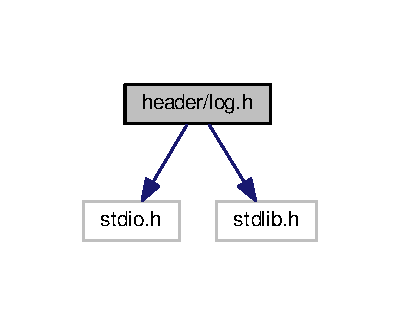
\includegraphics[width=192pt]{log_8h__incl}
\end{center}
\end{figure}
\subsection*{Functions}
\begin{DoxyCompactItemize}
\item 
void \hyperlink{log_8h_a15ceb2cd576e93eb17ff4892e4931e0e}{reset\+Log\+File} ()
\begin{DoxyCompactList}\small\item\em Méthode permettant de vider le fichier de log. \end{DoxyCompactList}\item 
void \hyperlink{log_8h_a8f199e8391f80633e1cf4853b473be97}{log\+Cmd} (char $\ast$cmd\+Line)
\begin{DoxyCompactList}\small\item\em Méthode permettant d\textquotesingle{}insérer une ligne dans le fichier de log. \end{DoxyCompactList}\end{DoxyCompactItemize}


\subsection{Detailed Description}
log header. 

\begin{DoxyAuthor}{Author}
vlambs 
\end{DoxyAuthor}
\begin{DoxyVersion}{Version}
0.\+1 
\end{DoxyVersion}
\begin{DoxyDate}{Date}
20180207
\end{DoxyDate}
Header principal. 

\subsection{Function Documentation}
\index{log.\+h@{log.\+h}!log\+Cmd@{log\+Cmd}}
\index{log\+Cmd@{log\+Cmd}!log.\+h@{log.\+h}}
\subsubsection[{\texorpdfstring{log\+Cmd(char $\ast$cmd\+Line)}{logCmd(char *cmdLine)}}]{\setlength{\rightskip}{0pt plus 5cm}char log\+Cmd (
\begin{DoxyParamCaption}
\item[{char $\ast$}]{cmd\+Line}
\end{DoxyParamCaption}
)}\hypertarget{log_8h_a8f199e8391f80633e1cf4853b473be97}{}\label{log_8h_a8f199e8391f80633e1cf4853b473be97}


Méthode permettant d\textquotesingle{}insérer une ligne dans le fichier de log. 

\begin{DoxyAuthor}{Author}
vlambs 
\end{DoxyAuthor}

\begin{DoxyParams}{Parameters}
{\em } & \\
\hline
\end{DoxyParams}
\index{log.\+h@{log.\+h}!reset\+Log\+File@{reset\+Log\+File}}
\index{reset\+Log\+File@{reset\+Log\+File}!log.\+h@{log.\+h}}
\subsubsection[{\texorpdfstring{reset\+Log\+File()}{resetLogFile()}}]{\setlength{\rightskip}{0pt plus 5cm}char reset\+Log\+File (
\begin{DoxyParamCaption}
{}
\end{DoxyParamCaption}
)}\hypertarget{log_8h_a15ceb2cd576e93eb17ff4892e4931e0e}{}\label{log_8h_a15ceb2cd576e93eb17ff4892e4931e0e}


Méthode permettant de vider le fichier de log. 

\begin{DoxyAuthor}{Author}
vlambs 
\end{DoxyAuthor}

\begin{DoxyParams}{Parameters}
{\em } & \\
\hline
\end{DoxyParams}

\hypertarget{shell_8h}{}\section{header/shell.h File Reference}
\label{shell_8h}\index{header/shell.\+h@{header/shell.\+h}}


Header principal.  


{\ttfamily \#include \char`\"{}typedef.\+h\char`\"{}}\\*
Include dependency graph for shell.\+h\+:\nopagebreak
\begin{figure}[H]
\begin{center}
\leavevmode
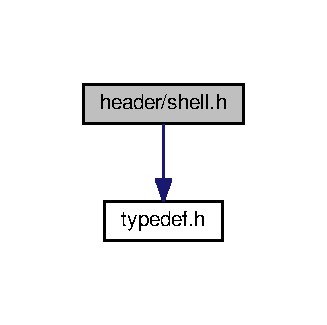
\includegraphics[width=157pt]{shell_8h__incl}
\end{center}
\end{figure}
\subsection*{Functions}
\begin{DoxyCompactItemize}
\item 
void \hyperlink{shell_8h_a4db33f9923b15a7b2fb2a61376a4d6ed}{add\+Alias} (char $\ast$input)
\begin{DoxyCompactList}\small\item\em Fonction permettant l\textquotesingle{}ajout d\textquotesingle{}un alias dans une Hash\+Map. \end{DoxyCompactList}\item 
char $\ast$ \hyperlink{shell_8h_a5d771f95c792771f6dafb7b8d7a8d5ed}{read\+Tree} (\hyperlink{struct__node}{node} $\ast$root)
\begin{DoxyCompactList}\small\item\em Fonction permettant de lire l\textquotesingle{}arbre de commande et de lancer le process des commandes. \end{DoxyCompactList}\item 
int \hyperlink{shell_8h_a3ae4caaca91ac9caf3a01901d969e39a}{run\+In\+Background} (char $\ast$complete\+Input, int index)
\begin{DoxyCompactList}\small\item\em Fonction permettant de lancer en arrière plan les commandes saisies. \end{DoxyCompactList}\item 
int \hyperlink{shell_8h_a248c40b7c05447d24a328de1833c81e1}{launch\+Process} (char $\ast$complete\+Input)
\begin{DoxyCompactList}\small\item\em Fonction permettant lancer la série de commande en avant plan. \end{DoxyCompactList}\item 
void \hyperlink{shell_8h_aed10a787c30b342e9f80f630376c50c0}{bash\+\_\+loop} (F\+I\+LE $\ast$f)
\begin{DoxyCompactList}\small\item\em Fonction permettant de boucler notre programme tant que la commande exit n\textquotesingle{}est pas entré par l\textquotesingle{}utilisateur. \end{DoxyCompactList}\end{DoxyCompactItemize}


\subsection{Detailed Description}
Header principal. 

\begin{DoxyAuthor}{Author}
lfreyss 
\end{DoxyAuthor}
\begin{DoxyVersion}{Version}
0.\+1 
\end{DoxyVersion}
\begin{DoxyDate}{Date}
24 janvier 2018
\end{DoxyDate}
Header principal. 

\subsection{Function Documentation}
\index{shell.\+h@{shell.\+h}!add\+Alias@{add\+Alias}}
\index{add\+Alias@{add\+Alias}!shell.\+h@{shell.\+h}}
\subsubsection[{\texorpdfstring{add\+Alias(char $\ast$input)}{addAlias(char *input)}}]{\setlength{\rightskip}{0pt plus 5cm}void add\+Alias (
\begin{DoxyParamCaption}
\item[{char $\ast$}]{input}
\end{DoxyParamCaption}
)}\hypertarget{shell_8h_a4db33f9923b15a7b2fb2a61376a4d6ed}{}\label{shell_8h_a4db33f9923b15a7b2fb2a61376a4d6ed}


Fonction permettant l\textquotesingle{}ajout d\textquotesingle{}un alias dans une Hash\+Map. 

\begin{DoxyAuthor}{Author}
lfreyss 
\end{DoxyAuthor}

\begin{DoxyParams}{Parameters}
{\em input} & -\/$>$ String entré par l\textquotesingle{}utilisateur commencant par la commande alias \\
\hline
\end{DoxyParams}
\begin{DoxyReturn}{Returns}

\end{DoxyReturn}
\index{shell.\+h@{shell.\+h}!bash\+\_\+loop@{bash\+\_\+loop}}
\index{bash\+\_\+loop@{bash\+\_\+loop}!shell.\+h@{shell.\+h}}
\subsubsection[{\texorpdfstring{bash\+\_\+loop(\+F\+I\+L\+E $\ast$f)}{bash_loop(FILE *f)}}]{\setlength{\rightskip}{0pt plus 5cm}void bash\+\_\+loop (
\begin{DoxyParamCaption}
\item[{F\+I\+LE $\ast$}]{f}
\end{DoxyParamCaption}
)}\hypertarget{shell_8h_aed10a787c30b342e9f80f630376c50c0}{}\label{shell_8h_aed10a787c30b342e9f80f630376c50c0}


Fonction permettant de boucler notre programme tant que la commande exit n\textquotesingle{}est pas entré par l\textquotesingle{}utilisateur. 

\begin{DoxyAuthor}{Author}
lfreyss 
\end{DoxyAuthor}

\begin{DoxyParams}{Parameters}
{\em fichier} & de log \\
\hline
\end{DoxyParams}
\begin{DoxyReturn}{Returns}

\end{DoxyReturn}
\index{shell.\+h@{shell.\+h}!launch\+Process@{launch\+Process}}
\index{launch\+Process@{launch\+Process}!shell.\+h@{shell.\+h}}
\subsubsection[{\texorpdfstring{launch\+Process(char $\ast$complete\+Input)}{launchProcess(char *completeInput)}}]{\setlength{\rightskip}{0pt plus 5cm}void launch\+Process (
\begin{DoxyParamCaption}
\item[{char $\ast$}]{complete\+Input}
\end{DoxyParamCaption}
)}\hypertarget{shell_8h_a248c40b7c05447d24a328de1833c81e1}{}\label{shell_8h_a248c40b7c05447d24a328de1833c81e1}


Fonction permettant lancer la série de commande en avant plan. 

\begin{DoxyAuthor}{Author}
lfreyss 
\end{DoxyAuthor}

\begin{DoxyParams}{Parameters}
{\em String} & contenant la saisie de l\textquotesingle{}entrée standard \\
\hline
\end{DoxyParams}
\begin{DoxyReturn}{Returns}
Statut du shell (doit quitter \+: 0; continuer la boucle\+: 1) 
\end{DoxyReturn}
\index{shell.\+h@{shell.\+h}!read\+Tree@{read\+Tree}}
\index{read\+Tree@{read\+Tree}!shell.\+h@{shell.\+h}}
\subsubsection[{\texorpdfstring{read\+Tree(node $\ast$root)}{readTree(node *root)}}]{\setlength{\rightskip}{0pt plus 5cm}char $\ast$ read\+Tree (
\begin{DoxyParamCaption}
\item[{{\bf node} $\ast$}]{root}
\end{DoxyParamCaption}
)}\hypertarget{shell_8h_a5d771f95c792771f6dafb7b8d7a8d5ed}{}\label{shell_8h_a5d771f95c792771f6dafb7b8d7a8d5ed}


Fonction permettant de lire l\textquotesingle{}arbre de commande et de lancer le process des commandes. 

\begin{DoxyAuthor}{Author}
lfreyss 
\end{DoxyAuthor}

\begin{DoxyParams}{Parameters}
{\em root} & -\/$>$ noeud principale de l\textquotesingle{}arbre \\
\hline
\end{DoxyParams}
\begin{DoxyReturn}{Returns}

\end{DoxyReturn}
\index{shell.\+h@{shell.\+h}!run\+In\+Background@{run\+In\+Background}}
\index{run\+In\+Background@{run\+In\+Background}!shell.\+h@{shell.\+h}}
\subsubsection[{\texorpdfstring{run\+In\+Background(char $\ast$complete\+Input, int index)}{runInBackground(char *completeInput, int index)}}]{\setlength{\rightskip}{0pt plus 5cm}int run\+In\+Background (
\begin{DoxyParamCaption}
\item[{char $\ast$}]{complete\+Input, }
\item[{int}]{index}
\end{DoxyParamCaption}
)}\hypertarget{shell_8h_a3ae4caaca91ac9caf3a01901d969e39a}{}\label{shell_8h_a3ae4caaca91ac9caf3a01901d969e39a}


Fonction permettant de lancer en arrière plan les commandes saisies. 

\begin{DoxyAuthor}{Author}
lfreyss 
\end{DoxyAuthor}

\begin{DoxyParams}{Parameters}
{\em String} & contenant la saisie de l\textquotesingle{}entrée standard, numéro d\textquotesingle{}index du char \& à retirer \\
\hline
\end{DoxyParams}
\begin{DoxyReturn}{Returns}

\end{DoxyReturn}

\hypertarget{tree_8h}{}\section{header/tree.h File Reference}
\label{tree_8h}\index{header/tree.\+h@{header/tree.\+h}}


librairie permettant l\textquotesingle{}utilisation d\textquotesingle{}un tree  


{\ttfamily \#include \char`\"{}typedef.\+h\char`\"{}}\\*
Include dependency graph for tree.\+h\+:\nopagebreak
\begin{figure}[H]
\begin{center}
\leavevmode
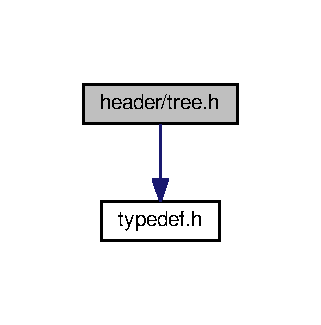
\includegraphics[width=154pt]{tree_8h__incl}
\end{center}
\end{figure}
\subsection*{Functions}
\begin{DoxyCompactItemize}
\item 
\hyperlink{typedef_8h_a1062901a7428fdd9c7f180f5e01ea056}{bool} \hyperlink{tree_8h_ab248547d5fd702c4cb2f35ba26013303}{is\+Operator} (char $\ast$c)
\begin{DoxyCompactList}\small\item\em Fonction permettant de déterminer si l\textquotesingle{}élément est un opérateur ou une commande. \end{DoxyCompactList}\item 
\hyperlink{struct__node}{node} $\ast$ \hyperlink{tree_8h_a36a86fd54baf613baa671435fe7488ae}{new\+Node} ()
\begin{DoxyCompactList}\small\item\em Fonction permettant la création d\textquotesingle{}un noeud vide. \end{DoxyCompactList}\item 
\hyperlink{struct__node}{node} $\ast$ \hyperlink{tree_8h_a13dd92c48cc266d1b1659ba98346f3aa}{construct\+Tree} (char $\ast$$\ast$input, int size\+Input)
\begin{DoxyCompactList}\small\item\em Fonction permettant de construire récursivement un arbre de commande. \end{DoxyCompactList}\item 
char $\ast$ \hyperlink{tree_8h_a2c958212afc71d4c61953776014b9ce6}{display\+Tree} (\hyperlink{struct__node}{node} $\ast$noeud)
\begin{DoxyCompactList}\small\item\em Fonction peremttant de visualiser dans la sortie standard un arbre à partir d\textquotesingle{}un noeud spécifique. \end{DoxyCompactList}\end{DoxyCompactItemize}


\subsection{Detailed Description}
librairie permettant l\textquotesingle{}utilisation d\textquotesingle{}un tree 

\begin{DoxyAuthor}{Author}
lfreyss 
\end{DoxyAuthor}
\begin{DoxyVersion}{Version}
0.\+1 
\end{DoxyVersion}
\begin{DoxyDate}{Date}
25 janvier 2018
\end{DoxyDate}
Définition des variables, enum, struct. 

\subsection{Function Documentation}
\index{tree.\+h@{tree.\+h}!construct\+Tree@{construct\+Tree}}
\index{construct\+Tree@{construct\+Tree}!tree.\+h@{tree.\+h}}
\subsubsection[{\texorpdfstring{construct\+Tree(char $\ast$$\ast$input, int size\+Input)}{constructTree(char **input, int sizeInput)}}]{\setlength{\rightskip}{0pt plus 5cm}{\bf node} $\ast$ construct\+Tree (
\begin{DoxyParamCaption}
\item[{char $\ast$$\ast$}]{input, }
\item[{int}]{size\+Input}
\end{DoxyParamCaption}
)}\hypertarget{tree_8h_a13dd92c48cc266d1b1659ba98346f3aa}{}\label{tree_8h_a13dd92c48cc266d1b1659ba98346f3aa}


Fonction permettant de construire récursivement un arbre de commande. 

\begin{DoxyAuthor}{Author}
lfreyss 
\end{DoxyAuthor}

\begin{DoxyParams}{Parameters}
{\em input} & -\/$>$ le tableau de string qu\textquotesingle{}il faut transformer en arbre, size\+Input -\/$>$ le nombre d\textquotesingle{}élément dans le tableau \\
\hline
\end{DoxyParams}
\begin{DoxyReturn}{Returns}
Le noeud construit lors de l\textquotesingle{}itération de récursivité 
\end{DoxyReturn}
\index{tree.\+h@{tree.\+h}!display\+Tree@{display\+Tree}}
\index{display\+Tree@{display\+Tree}!tree.\+h@{tree.\+h}}
\subsubsection[{\texorpdfstring{display\+Tree(node $\ast$noeud)}{displayTree(node *noeud)}}]{\setlength{\rightskip}{0pt plus 5cm}char $\ast$ display\+Tree (
\begin{DoxyParamCaption}
\item[{{\bf node} $\ast$}]{noeud}
\end{DoxyParamCaption}
)}\hypertarget{tree_8h_a2c958212afc71d4c61953776014b9ce6}{}\label{tree_8h_a2c958212afc71d4c61953776014b9ce6}


Fonction peremttant de visualiser dans la sortie standard un arbre à partir d\textquotesingle{}un noeud spécifique. 

\begin{DoxyAuthor}{Author}
lfreyss 
\end{DoxyAuthor}

\begin{DoxyParams}{Parameters}
{\em Noeud} & spécifique à partir du quel on affiche l\textquotesingle{}arbre \\
\hline
\end{DoxyParams}
\begin{DoxyReturn}{Returns}
valeur du noeud 
\end{DoxyReturn}
\index{tree.\+h@{tree.\+h}!is\+Operator@{is\+Operator}}
\index{is\+Operator@{is\+Operator}!tree.\+h@{tree.\+h}}
\subsubsection[{\texorpdfstring{is\+Operator(char $\ast$c)}{isOperator(char *c)}}]{\setlength{\rightskip}{0pt plus 5cm}{\bf bool} is\+Operator (
\begin{DoxyParamCaption}
\item[{char $\ast$}]{c}
\end{DoxyParamCaption}
)}\hypertarget{tree_8h_ab248547d5fd702c4cb2f35ba26013303}{}\label{tree_8h_ab248547d5fd702c4cb2f35ba26013303}


Fonction permettant de déterminer si l\textquotesingle{}élément est un opérateur ou une commande. 

\begin{DoxyAuthor}{Author}
lfreyss 
\end{DoxyAuthor}

\begin{DoxyParams}{Parameters}
{\em c} & -\/$>$ élément à examiner \\
\hline
\end{DoxyParams}
\begin{DoxyReturn}{Returns}
est un opérateur ou non 
\end{DoxyReturn}
\index{tree.\+h@{tree.\+h}!new\+Node@{new\+Node}}
\index{new\+Node@{new\+Node}!tree.\+h@{tree.\+h}}
\subsubsection[{\texorpdfstring{new\+Node()}{newNode()}}]{\setlength{\rightskip}{0pt plus 5cm}{\bf node} $\ast$ new\+Node (
\begin{DoxyParamCaption}
{}
\end{DoxyParamCaption}
)}\hypertarget{tree_8h_a36a86fd54baf613baa671435fe7488ae}{}\label{tree_8h_a36a86fd54baf613baa671435fe7488ae}


Fonction permettant la création d\textquotesingle{}un noeud vide. 

\begin{DoxyAuthor}{Author}
lfreyss 
\end{DoxyAuthor}

\begin{DoxyParams}{Parameters}
{\em } & \\
\hline
\end{DoxyParams}

\hypertarget{typedef_8h}{}\section{header/typedef.h File Reference}
\label{typedef_8h}\index{header/typedef.\+h@{header/typedef.\+h}}


Définition des variables, enum, struct.  


This graph shows which files directly or indirectly include this file\+:\nopagebreak
\begin{figure}[H]
\begin{center}
\leavevmode
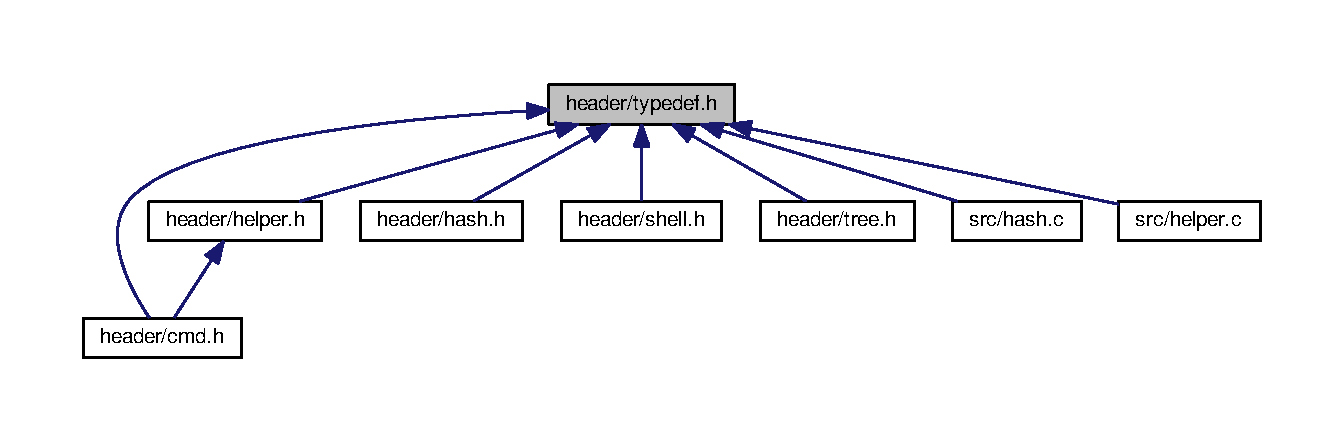
\includegraphics[width=350pt]{typedef_8h__dep__incl}
\end{center}
\end{figure}
\subsection*{Classes}
\begin{DoxyCompactItemize}
\item 
struct \hyperlink{struct__node}{\+\_\+node}
\item 
struct \hyperlink{structnlist}{nlist}
\end{DoxyCompactItemize}
\subsection*{Macros}
\begin{DoxyCompactItemize}
\item 
\#define {\bfseries true}~1\hypertarget{typedef_8h_a41f9c5fb8b08eb5dc3edce4dcb37fee7}{}\label{typedef_8h_a41f9c5fb8b08eb5dc3edce4dcb37fee7}

\item 
\#define {\bfseries false}~0\hypertarget{typedef_8h_a65e9886d74aaee76545e83dd09011727}{}\label{typedef_8h_a65e9886d74aaee76545e83dd09011727}

\end{DoxyCompactItemize}
\subsection*{Typedefs}
\begin{DoxyCompactItemize}
\item 
typedef struct \hyperlink{struct__node}{\+\_\+node} {\bfseries node}\hypertarget{typedef_8h_addb697c9bca6f8981a870daa4953af4f}{}\label{typedef_8h_addb697c9bca6f8981a870daa4953af4f}

\item 
typedef int \hyperlink{typedef_8h_a1062901a7428fdd9c7f180f5e01ea056}{bool}
\begin{DoxyCompactList}\small\item\em Structure permettant l\textquotesingle{}utilisation de boolean. \end{DoxyCompactList}\end{DoxyCompactItemize}


\subsection{Detailed Description}
Définition des variables, enum, struct. 

\begin{DoxyAuthor}{Author}
vlambs 
\end{DoxyAuthor}
\begin{DoxyVersion}{Version}
0.\+1 
\end{DoxyVersion}
\begin{DoxyDate}{Date}
24 janvier 2018
\end{DoxyDate}
Définition des variables, enum, struct. 

\subsection{Typedef Documentation}
\index{typedef.\+h@{typedef.\+h}!bool@{bool}}
\index{bool@{bool}!typedef.\+h@{typedef.\+h}}
\subsubsection[{\texorpdfstring{bool}{bool}}]{\setlength{\rightskip}{0pt plus 5cm}typedef int {\bf bool}}\hypertarget{typedef_8h_a1062901a7428fdd9c7f180f5e01ea056}{}\label{typedef_8h_a1062901a7428fdd9c7f180f5e01ea056}


Structure permettant l\textquotesingle{}utilisation de boolean. 

\begin{DoxyAuthor}{Author}
lfreyss 
\end{DoxyAuthor}

\hypertarget{hash_8c}{}\section{src/hash.c File Reference}
\label{hash_8c}\index{src/hash.\+c@{src/hash.\+c}}


Fichier contenant les fonctions utiles à un Hash\+Map. Code source venant de Section 6.\+6 of The C Programming Language.  


{\ttfamily \#include $<$stdlib.\+h$>$}\\*
{\ttfamily \#include $<$stdio.\+h$>$}\\*
{\ttfamily \#include $<$string.\+h$>$}\\*
{\ttfamily \#include \char`\"{}../header/typedef.\+h\char`\"{}}\\*
Include dependency graph for hash.\+c\+:\nopagebreak
\begin{figure}[H]
\begin{center}
\leavevmode
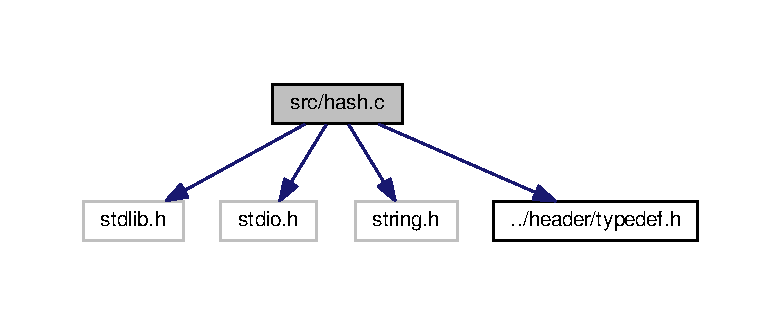
\includegraphics[width=350pt]{hash_8c__incl}
\end{center}
\end{figure}
\subsection*{Macros}
\begin{DoxyCompactItemize}
\item 
\#define {\bfseries H\+A\+S\+H\+S\+I\+ZE}~101\hypertarget{hash_8c_a2b4054af9a8f1ec4104846747ded1675}{}\label{hash_8c_a2b4054af9a8f1ec4104846747ded1675}

\end{DoxyCompactItemize}
\subsection*{Functions}
\begin{DoxyCompactItemize}
\item 
unsigned {\bfseries hash} (char $\ast$s)\hypertarget{hash_8c_a998ad9aa6cfe8a43b60cdc806667bdb2}{}\label{hash_8c_a998ad9aa6cfe8a43b60cdc806667bdb2}

\item 
struct \hyperlink{structnlist}{nlist} $\ast$ \hyperlink{hash_8c_a26fc137872cf2f9e5741b30a7ed6670f}{lookup} (char $\ast$s)
\begin{DoxyCompactList}\small\item\em Fonction permettant de parcourir la Hash\+Map et de trouver l\textquotesingle{}élement voulu. \end{DoxyCompactList}\item 
struct \hyperlink{structnlist}{nlist} $\ast$ \hyperlink{hash_8c_a94f41788b6c7255236e7a28b1ea71580}{install} (char $\ast$name, char $\ast$defn)
\begin{DoxyCompactList}\small\item\em Fonction permettant de rajouter un élément à la Hash\+Map. \end{DoxyCompactList}\end{DoxyCompactItemize}


\subsection{Detailed Description}
Fichier contenant les fonctions utiles à un Hash\+Map. Code source venant de Section 6.\+6 of The C Programming Language. 

\begin{DoxyAuthor}{Author}
lfreyss 
\end{DoxyAuthor}
\begin{DoxyVersion}{Version}
0.\+1 
\end{DoxyVersion}
\begin{DoxyDate}{Date}
20180308
\end{DoxyDate}
Fichier contenant les fonctionnalités H\+A\+SH . 

\subsection{Function Documentation}
\index{hash.\+c@{hash.\+c}!install@{install}}
\index{install@{install}!hash.\+c@{hash.\+c}}
\subsubsection[{\texorpdfstring{install(char $\ast$name, char $\ast$defn)}{install(char *name, char *defn)}}]{\setlength{\rightskip}{0pt plus 5cm}struct {\bf nlist}$\ast$ install (
\begin{DoxyParamCaption}
\item[{char $\ast$}]{name, }
\item[{char $\ast$}]{defn}
\end{DoxyParamCaption}
)}\hypertarget{hash_8c_a94f41788b6c7255236e7a28b1ea71580}{}\label{hash_8c_a94f41788b6c7255236e7a28b1ea71580}


Fonction permettant de rajouter un élément à la Hash\+Map. 

\begin{DoxyAuthor}{Author}
lfreyss 
\end{DoxyAuthor}

\begin{DoxyParams}{Parameters}
{\em name} & -\/$>$ nom du hashmap; defn -\/$>$ valeur du hashmap \\
\hline
\end{DoxyParams}
\begin{DoxyReturn}{Returns}
nlist que l\textquotesingle{}on vient de rajouter 
\end{DoxyReturn}
\index{hash.\+c@{hash.\+c}!lookup@{lookup}}
\index{lookup@{lookup}!hash.\+c@{hash.\+c}}
\subsubsection[{\texorpdfstring{lookup(char $\ast$s)}{lookup(char *s)}}]{\setlength{\rightskip}{0pt plus 5cm}struct {\bf nlist}$\ast$ lookup (
\begin{DoxyParamCaption}
\item[{char $\ast$}]{s}
\end{DoxyParamCaption}
)}\hypertarget{hash_8c_a26fc137872cf2f9e5741b30a7ed6670f}{}\label{hash_8c_a26fc137872cf2f9e5741b30a7ed6670f}


Fonction permettant de parcourir la Hash\+Map et de trouver l\textquotesingle{}élement voulu. 

\begin{DoxyAuthor}{Author}
lfreyss 
\end{DoxyAuthor}

\begin{DoxyParams}{Parameters}
{\em chaine} & de caractère que l\textquotesingle{}on recherche \\
\hline
\end{DoxyParams}
\begin{DoxyReturn}{Returns}
Struct nlist recherchée ou null si non trouvée 
\end{DoxyReturn}

\hypertarget{helper_8c}{}\section{src/helper.c File Reference}
\label{helper_8c}\index{src/helper.\+c@{src/helper.\+c}}


Fichier contenant les fonctions d\textquotesingle{}helper.  


{\ttfamily \#include $<$stdlib.\+h$>$}\\*
{\ttfamily \#include $<$stdio.\+h$>$}\\*
{\ttfamily \#include $<$string.\+h$>$}\\*
{\ttfamily \#include \char`\"{}../header/typedef.\+h\char`\"{}}\\*
Include dependency graph for helper.\+c\+:\nopagebreak
\begin{figure}[H]
\begin{center}
\leavevmode
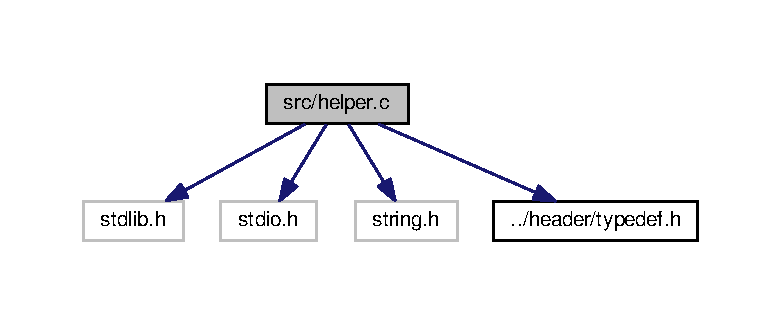
\includegraphics[width=350pt]{helper_8c__incl}
\end{center}
\end{figure}
\subsection*{Functions}
\begin{DoxyCompactItemize}
\item 
char $\ast$ \hyperlink{helper_8c_a4ac40b6eb62ee09336c690894977841a}{readline} (void)
\begin{DoxyCompactList}\small\item\em Fonction permettant de lire la saisie de l\textquotesingle{}entrée standard. \end{DoxyCompactList}\item 
int \hyperlink{helper_8c_a1e941fcaa0b19e24f436561f13fff047}{parse\+Space} (char $\ast$str, char $\ast$parsed\mbox{[}$\,$\mbox{]})
\begin{DoxyCompactList}\small\item\em Fonction permettant de séparer une chaine de caractère par des espaces. \end{DoxyCompactList}\item 
int \hyperlink{helper_8c_a1db78452432b56ef399a0b054b62a638}{parse\+String} (char $\ast$str, char $\ast$parsed\mbox{[}$\,$\mbox{]}, char $\ast$sep)
\begin{DoxyCompactList}\small\item\em Fonction permettant de séparer une chaine de caractère par un caractère pré-\/définie. \end{DoxyCompactList}\item 
void \hyperlink{helper_8c_a1d9ff13ca6fbfeed019ff8459a2d7b27}{ltrim} (char $\ast$str)
\begin{DoxyCompactList}\small\item\em Fonction permettant de supprimer les espaces, les tabulations et sauts de ligne en début de string. \end{DoxyCompactList}\item 
void \hyperlink{helper_8c_a36c31afc53e5a1e87177eff988d6d17e}{rtrim} (char $\ast$str)
\begin{DoxyCompactList}\small\item\em Fonction permettant de supprimer les espaces, les tabulations et sauts de ligne en fin de string. \end{DoxyCompactList}\item 
void \hyperlink{helper_8c_a67a5c19d5a2782a49836a0b9190b88f8}{trim} (char str\mbox{[}$\,$\mbox{]})
\begin{DoxyCompactList}\small\item\em Fonction permettant d\textquotesingle{}appeler le rtrim et ltrim en un seul appel. \end{DoxyCompactList}\item 
void \hyperlink{helper_8c_a18c4769c27205c182ebca5ff7499c1ab}{add\+Char} (char c, char $\ast$string\+To\+Add)
\begin{DoxyCompactList}\small\item\em Concatène un caractère à une chaine de caractère. \end{DoxyCompactList}\item 
int \hyperlink{helper_8c_a6dc328bf1c07bf8d8c87aab9ab66658f}{parse\+Control\+Operator} (char $\ast$str, char $\ast$$\ast$parsed)
\begin{DoxyCompactList}\small\item\em Fonction permettant de découper une string par les opérateurs de control, à savoir \&\& et $\vert$$\vert$. \end{DoxyCompactList}\item 
int \hyperlink{helper_8c_a983ac2428db05783a35c1341febb9d37}{parse\+Redirection\+Flux} (char $\ast$str, char $\ast$$\ast$parsed)
\begin{DoxyCompactList}\small\item\em Fonction permettant de découper une string par les opérateurs de redirection de flux, à savoir $\vert$,\&,$<$,$>$,$<$$<$,$>$$>$ \end{DoxyCompactList}\item 
char $\ast$$\ast$ \hyperlink{helper_8c_a7e3caf7b27708ecf1215a42ab4ebfe91}{create\+Calloc\+Tab} (int x, int y)
\begin{DoxyCompactList}\small\item\em Fonction permettant de créer un tableau de chaine de caractère. \end{DoxyCompactList}\item 
void \hyperlink{helper_8c_a00eacdb7422e4261253801a228a102a0}{copy\+Content\+File} (char $\ast$writefilename, char $\ast$readfilename, \hyperlink{typedef_8h_a1062901a7428fdd9c7f180f5e01ea056}{bool} overide)
\begin{DoxyCompactList}\small\item\em Fonction permettant la copie du contenu d\textquotesingle{}un fichier vers un autre. \end{DoxyCompactList}\item 
\hyperlink{typedef_8h_a1062901a7428fdd9c7f180f5e01ea056}{bool} \hyperlink{helper_8c_a9b39605351f88642b3f802a77a607185}{file\+Is\+Empty} ()
\begin{DoxyCompactList}\small\item\em Fonction permettant de check si un fichier est vide ou non. \end{DoxyCompactList}\item 
void \hyperlink{helper_8c_aaebc21a8340b94ee50729f1d95a3b389}{display\+Output} (char $\ast$filename)
\begin{DoxyCompactList}\small\item\em Fonction permettant de afficher le contenu d\textquotesingle{}un fichier sur la sortie standard. \end{DoxyCompactList}\item 
void \hyperlink{helper_8c_a91810b2c3cb895cb752b64be77c8c4a1}{add\+Content\+To\+File} (char $\ast$str)
\begin{DoxyCompactList}\small\item\em Fonction permettant de rajouter du contenu à un fichier. \end{DoxyCompactList}\end{DoxyCompactItemize}


\subsection{Detailed Description}
Fichier contenant les fonctions d\textquotesingle{}helper. 

\begin{DoxyAuthor}{Author}
lfreyss 
\end{DoxyAuthor}
\begin{DoxyVersion}{Version}
0.\+1 
\end{DoxyVersion}
\begin{DoxyDate}{Date}
20180207
\end{DoxyDate}
Fichier contenant les fonctionnalité . 

\subsection{Function Documentation}
\index{helper.\+c@{helper.\+c}!add\+Char@{add\+Char}}
\index{add\+Char@{add\+Char}!helper.\+c@{helper.\+c}}
\subsubsection[{\texorpdfstring{add\+Char(char c, char $\ast$string\+To\+Add)}{addChar(char c, char *stringToAdd)}}]{\setlength{\rightskip}{0pt plus 5cm}void add\+Char (
\begin{DoxyParamCaption}
\item[{char}]{c, }
\item[{char $\ast$}]{string\+To\+Add}
\end{DoxyParamCaption}
)}\hypertarget{helper_8c_a18c4769c27205c182ebca5ff7499c1ab}{}\label{helper_8c_a18c4769c27205c182ebca5ff7499c1ab}


Concatène un caractère à une chaine de caractère. 

\begin{DoxyAuthor}{Author}
lfreyss 
\end{DoxyAuthor}

\begin{DoxyParams}{Parameters}
{\em Caractère} & à concatèner, chaine de caractère à concatèner \\
\hline
\end{DoxyParams}
\begin{DoxyReturn}{Returns}

\end{DoxyReturn}
\index{helper.\+c@{helper.\+c}!add\+Content\+To\+File@{add\+Content\+To\+File}}
\index{add\+Content\+To\+File@{add\+Content\+To\+File}!helper.\+c@{helper.\+c}}
\subsubsection[{\texorpdfstring{add\+Content\+To\+File(char $\ast$str)}{addContentToFile(char *str)}}]{\setlength{\rightskip}{0pt plus 5cm}void add\+Content\+To\+File (
\begin{DoxyParamCaption}
\item[{char $\ast$}]{str}
\end{DoxyParamCaption}
)}\hypertarget{helper_8c_a91810b2c3cb895cb752b64be77c8c4a1}{}\label{helper_8c_a91810b2c3cb895cb752b64be77c8c4a1}


Fonction permettant de rajouter du contenu à un fichier. 

\begin{DoxyAuthor}{Author}
lfreyss 
\end{DoxyAuthor}

\begin{DoxyParams}{Parameters}
{\em String} & à ajouter au contenu du fichier \\
\hline
\end{DoxyParams}
\begin{DoxyReturn}{Returns}

\end{DoxyReturn}
\index{helper.\+c@{helper.\+c}!copy\+Content\+File@{copy\+Content\+File}}
\index{copy\+Content\+File@{copy\+Content\+File}!helper.\+c@{helper.\+c}}
\subsubsection[{\texorpdfstring{copy\+Content\+File(char $\ast$writefilename, char $\ast$readfilename, bool overide)}{copyContentFile(char *writefilename, char *readfilename, bool overide)}}]{\setlength{\rightskip}{0pt plus 5cm}void copy\+Content\+File (
\begin{DoxyParamCaption}
\item[{char $\ast$}]{writefilename, }
\item[{char $\ast$}]{readfilename, }
\item[{{\bf bool}}]{overide}
\end{DoxyParamCaption}
)}\hypertarget{helper_8c_a00eacdb7422e4261253801a228a102a0}{}\label{helper_8c_a00eacdb7422e4261253801a228a102a0}


Fonction permettant la copie du contenu d\textquotesingle{}un fichier vers un autre. 

\begin{DoxyAuthor}{Author}
lfreyss 
\end{DoxyAuthor}

\begin{DoxyParams}{Parameters}
{\em writefilename} & -\/$>$ fichier de destination, readfilename -\/$>$ fichier source, overide -\/$>$ ajouter au contenu ou le remplacer \\
\hline
\end{DoxyParams}
\begin{DoxyReturn}{Returns}

\end{DoxyReturn}
\index{helper.\+c@{helper.\+c}!create\+Calloc\+Tab@{create\+Calloc\+Tab}}
\index{create\+Calloc\+Tab@{create\+Calloc\+Tab}!helper.\+c@{helper.\+c}}
\subsubsection[{\texorpdfstring{create\+Calloc\+Tab(int x, int y)}{createCallocTab(int x, int y)}}]{\setlength{\rightskip}{0pt plus 5cm}char$\ast$$\ast$ create\+Calloc\+Tab (
\begin{DoxyParamCaption}
\item[{int}]{x, }
\item[{int}]{y}
\end{DoxyParamCaption}
)}\hypertarget{helper_8c_a7e3caf7b27708ecf1215a42ab4ebfe91}{}\label{helper_8c_a7e3caf7b27708ecf1215a42ab4ebfe91}


Fonction permettant de créer un tableau de chaine de caractère. 

\begin{DoxyAuthor}{Author}
lfreyss 
\end{DoxyAuthor}

\begin{DoxyParams}{Parameters}
{\em x} & -\/$>$ nombre de chaine de caractère, y -\/$>$ nombre de caractère dans une chaine de caractère \\
\hline
\end{DoxyParams}
\begin{DoxyReturn}{Returns}
Le tableau de chaine de caractère 
\end{DoxyReturn}
\index{helper.\+c@{helper.\+c}!display\+Output@{display\+Output}}
\index{display\+Output@{display\+Output}!helper.\+c@{helper.\+c}}
\subsubsection[{\texorpdfstring{display\+Output(char $\ast$filename)}{displayOutput(char *filename)}}]{\setlength{\rightskip}{0pt plus 5cm}void display\+Output (
\begin{DoxyParamCaption}
\item[{char $\ast$}]{filename}
\end{DoxyParamCaption}
)}\hypertarget{helper_8c_aaebc21a8340b94ee50729f1d95a3b389}{}\label{helper_8c_aaebc21a8340b94ee50729f1d95a3b389}


Fonction permettant de afficher le contenu d\textquotesingle{}un fichier sur la sortie standard. 

\begin{DoxyAuthor}{Author}
lfreyss 
\end{DoxyAuthor}

\begin{DoxyParams}{Parameters}
{\em Nom} & du fichier \\
\hline
\end{DoxyParams}
\begin{DoxyReturn}{Returns}

\end{DoxyReturn}
\index{helper.\+c@{helper.\+c}!file\+Is\+Empty@{file\+Is\+Empty}}
\index{file\+Is\+Empty@{file\+Is\+Empty}!helper.\+c@{helper.\+c}}
\subsubsection[{\texorpdfstring{file\+Is\+Empty()}{fileIsEmpty()}}]{\setlength{\rightskip}{0pt plus 5cm}{\bf bool} file\+Is\+Empty (
\begin{DoxyParamCaption}
{}
\end{DoxyParamCaption}
)}\hypertarget{helper_8c_a9b39605351f88642b3f802a77a607185}{}\label{helper_8c_a9b39605351f88642b3f802a77a607185}


Fonction permettant de check si un fichier est vide ou non. 

\begin{DoxyAuthor}{Author}
lfreyss 
\end{DoxyAuthor}

\begin{DoxyParams}{Parameters}
{\em } & \\
\hline
\end{DoxyParams}
\index{helper.\+c@{helper.\+c}!ltrim@{ltrim}}
\index{ltrim@{ltrim}!helper.\+c@{helper.\+c}}
\subsubsection[{\texorpdfstring{ltrim(char $\ast$str)}{ltrim(char *str)}}]{\setlength{\rightskip}{0pt plus 5cm}void ltrim (
\begin{DoxyParamCaption}
\item[{char $\ast$}]{str}
\end{DoxyParamCaption}
)}\hypertarget{helper_8c_a1d9ff13ca6fbfeed019ff8459a2d7b27}{}\label{helper_8c_a1d9ff13ca6fbfeed019ff8459a2d7b27}


Fonction permettant de supprimer les espaces, les tabulations et sauts de ligne en début de string. 

\begin{DoxyAuthor}{Author}
lfreyss 
\end{DoxyAuthor}

\begin{DoxyParams}{Parameters}
{\em String} & à examiner \\
\hline
\end{DoxyParams}
\begin{DoxyReturn}{Returns}

\end{DoxyReturn}
\index{helper.\+c@{helper.\+c}!parse\+Control\+Operator@{parse\+Control\+Operator}}
\index{parse\+Control\+Operator@{parse\+Control\+Operator}!helper.\+c@{helper.\+c}}
\subsubsection[{\texorpdfstring{parse\+Control\+Operator(char $\ast$str, char $\ast$$\ast$parsed)}{parseControlOperator(char *str, char **parsed)}}]{\setlength{\rightskip}{0pt plus 5cm}int parse\+Control\+Operator (
\begin{DoxyParamCaption}
\item[{char $\ast$}]{str, }
\item[{char $\ast$$\ast$}]{parsed}
\end{DoxyParamCaption}
)}\hypertarget{helper_8c_a6dc328bf1c07bf8d8c87aab9ab66658f}{}\label{helper_8c_a6dc328bf1c07bf8d8c87aab9ab66658f}


Fonction permettant de découper une string par les opérateurs de control, à savoir \&\& et $\vert$$\vert$. 

\begin{DoxyAuthor}{Author}
lfreyss 
\end{DoxyAuthor}

\begin{DoxyParams}{Parameters}
{\em String} & a découper, tab de string contenant la chaine de caractère découpé \\
\hline
\end{DoxyParams}
\begin{DoxyReturn}{Returns}
nombre de string dans le tableau 
\end{DoxyReturn}
\index{helper.\+c@{helper.\+c}!parse\+Redirection\+Flux@{parse\+Redirection\+Flux}}
\index{parse\+Redirection\+Flux@{parse\+Redirection\+Flux}!helper.\+c@{helper.\+c}}
\subsubsection[{\texorpdfstring{parse\+Redirection\+Flux(char $\ast$str, char $\ast$$\ast$parsed)}{parseRedirectionFlux(char *str, char **parsed)}}]{\setlength{\rightskip}{0pt plus 5cm}int parse\+Redirection\+Flux (
\begin{DoxyParamCaption}
\item[{char $\ast$}]{str, }
\item[{char $\ast$$\ast$}]{parsed}
\end{DoxyParamCaption}
)}\hypertarget{helper_8c_a983ac2428db05783a35c1341febb9d37}{}\label{helper_8c_a983ac2428db05783a35c1341febb9d37}


Fonction permettant de découper une string par les opérateurs de redirection de flux, à savoir $\vert$,\&,$<$,$>$,$<$$<$,$>$$>$ 

\begin{DoxyAuthor}{Author}
lfreyss 
\end{DoxyAuthor}

\begin{DoxyParams}{Parameters}
{\em String} & a découper, tab de string contenant la chaine de caractère découpé \\
\hline
\end{DoxyParams}
\begin{DoxyReturn}{Returns}
nombre de string dans le tableau 
\end{DoxyReturn}
\index{helper.\+c@{helper.\+c}!parse\+Space@{parse\+Space}}
\index{parse\+Space@{parse\+Space}!helper.\+c@{helper.\+c}}
\subsubsection[{\texorpdfstring{parse\+Space(char $\ast$str, char $\ast$parsed[])}{parseSpace(char *str, char *parsed[])}}]{\setlength{\rightskip}{0pt plus 5cm}int parse\+Space (
\begin{DoxyParamCaption}
\item[{char $\ast$}]{str, }
\item[{char $\ast$}]{parsed\mbox{[}$\,$\mbox{]}}
\end{DoxyParamCaption}
)}\hypertarget{helper_8c_a1e941fcaa0b19e24f436561f13fff047}{}\label{helper_8c_a1e941fcaa0b19e24f436561f13fff047}


Fonction permettant de séparer une chaine de caractère par des espaces. 

\begin{DoxyAuthor}{Author}
lfreyss 
\end{DoxyAuthor}

\begin{DoxyParams}{Parameters}
{\em str} & -\/$>$ chaine de caractère à séparer; parsed\mbox{[}\mbox{]} -\/$>$ tab de string contenant les string séprarés \\
\hline
\end{DoxyParams}
\begin{DoxyReturn}{Returns}

\end{DoxyReturn}
\index{helper.\+c@{helper.\+c}!parse\+String@{parse\+String}}
\index{parse\+String@{parse\+String}!helper.\+c@{helper.\+c}}
\subsubsection[{\texorpdfstring{parse\+String(char $\ast$str, char $\ast$parsed[], char $\ast$sep)}{parseString(char *str, char *parsed[], char *sep)}}]{\setlength{\rightskip}{0pt plus 5cm}int parse\+String (
\begin{DoxyParamCaption}
\item[{char $\ast$}]{str, }
\item[{char $\ast$}]{parsed\mbox{[}$\,$\mbox{]}, }
\item[{char $\ast$}]{sep}
\end{DoxyParamCaption}
)}\hypertarget{helper_8c_a1db78452432b56ef399a0b054b62a638}{}\label{helper_8c_a1db78452432b56ef399a0b054b62a638}


Fonction permettant de séparer une chaine de caractère par un caractère pré-\/définie. 

\begin{DoxyAuthor}{Author}
lfreyss 
\end{DoxyAuthor}

\begin{DoxyParams}{Parameters}
{\em str} & -\/$>$ chaine de caractère à séparer; parsed\mbox{[}\mbox{]} -\/$>$ tab de string contenant les string séprarés, sep -\/$>$ char de sépération \\
\hline
\end{DoxyParams}
\begin{DoxyReturn}{Returns}

\end{DoxyReturn}
\index{helper.\+c@{helper.\+c}!readline@{readline}}
\index{readline@{readline}!helper.\+c@{helper.\+c}}
\subsubsection[{\texorpdfstring{readline(void)}{readline(void)}}]{\setlength{\rightskip}{0pt plus 5cm}char$\ast$ readline (
\begin{DoxyParamCaption}
\item[{void}]{}
\end{DoxyParamCaption}
)}\hypertarget{helper_8c_a4ac40b6eb62ee09336c690894977841a}{}\label{helper_8c_a4ac40b6eb62ee09336c690894977841a}


Fonction permettant de lire la saisie de l\textquotesingle{}entrée standard. 

\begin{DoxyAuthor}{Author}
lfreyss 
\end{DoxyAuthor}

\begin{DoxyParams}{Parameters}
{\em } & \\
\hline
\end{DoxyParams}
\index{helper.\+c@{helper.\+c}!rtrim@{rtrim}}
\index{rtrim@{rtrim}!helper.\+c@{helper.\+c}}
\subsubsection[{\texorpdfstring{rtrim(char $\ast$str)}{rtrim(char *str)}}]{\setlength{\rightskip}{0pt plus 5cm}void rtrim (
\begin{DoxyParamCaption}
\item[{char $\ast$}]{str}
\end{DoxyParamCaption}
)}\hypertarget{helper_8c_a36c31afc53e5a1e87177eff988d6d17e}{}\label{helper_8c_a36c31afc53e5a1e87177eff988d6d17e}


Fonction permettant de supprimer les espaces, les tabulations et sauts de ligne en fin de string. 

\begin{DoxyAuthor}{Author}
lfreyss 
\end{DoxyAuthor}

\begin{DoxyParams}{Parameters}
{\em String} & à examiner \\
\hline
\end{DoxyParams}
\begin{DoxyReturn}{Returns}

\end{DoxyReturn}
\index{helper.\+c@{helper.\+c}!trim@{trim}}
\index{trim@{trim}!helper.\+c@{helper.\+c}}
\subsubsection[{\texorpdfstring{trim(char str[])}{trim(char str[])}}]{\setlength{\rightskip}{0pt plus 5cm}void trim (
\begin{DoxyParamCaption}
\item[{char}]{str\mbox{[}$\,$\mbox{]}}
\end{DoxyParamCaption}
)}\hypertarget{helper_8c_a67a5c19d5a2782a49836a0b9190b88f8}{}\label{helper_8c_a67a5c19d5a2782a49836a0b9190b88f8}


Fonction permettant d\textquotesingle{}appeler le rtrim et ltrim en un seul appel. 

\begin{DoxyAuthor}{Author}
lfreyss 
\end{DoxyAuthor}

\begin{DoxyParams}{Parameters}
{\em String} & à examiner \\
\hline
\end{DoxyParams}
\begin{DoxyReturn}{Returns}

\end{DoxyReturn}

\hypertarget{log_8c}{}\section{src/log.c File Reference}
\label{log_8c}\index{src/log.\+c@{src/log.\+c}}


Interaction fichier log.  


{\ttfamily \#include $<$stdio.\+h$>$}\\*
{\ttfamily \#include $<$stdlib.\+h$>$}\\*
Include dependency graph for log.\+c\+:\nopagebreak
\begin{figure}[H]
\begin{center}
\leavevmode
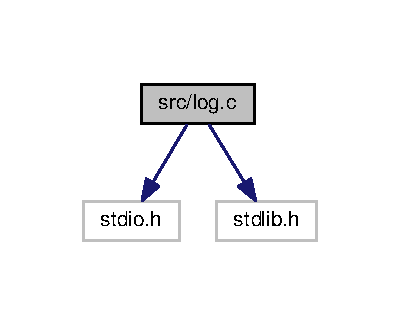
\includegraphics[width=192pt]{log_8c__incl}
\end{center}
\end{figure}
\subsection*{Functions}
\begin{DoxyCompactItemize}
\item 
void \hyperlink{log_8c_a03cfb949bc7889127d3e1e1693a0b2f2}{log\+Cmd} (char $\ast$cmd\+Line)
\begin{DoxyCompactList}\small\item\em Méthode permettant d\textquotesingle{}insérer une ligne dans le fichier de log. \end{DoxyCompactList}\item 
void \hyperlink{log_8c_a0dab74852bdd1cc8c4e5f4dc13a7ed6c}{reset\+Log\+File} ()
\begin{DoxyCompactList}\small\item\em Méthode permettant de vider le fichier de log. \end{DoxyCompactList}\end{DoxyCompactItemize}


\subsection{Detailed Description}
Interaction fichier log. 

\begin{DoxyAuthor}{Author}
vlambs 
\end{DoxyAuthor}
\begin{DoxyVersion}{Version}
0.\+1 
\end{DoxyVersion}
\begin{DoxyDate}{Date}
07 mars 2018
\end{DoxyDate}
Classe d\textquotesingle{}interaction avec fichier de log. 

\subsection{Function Documentation}
\index{log.\+c@{log.\+c}!log\+Cmd@{log\+Cmd}}
\index{log\+Cmd@{log\+Cmd}!log.\+c@{log.\+c}}
\subsubsection[{\texorpdfstring{log\+Cmd(char $\ast$cmd\+Line)}{logCmd(char *cmdLine)}}]{\setlength{\rightskip}{0pt plus 5cm}void log\+Cmd (
\begin{DoxyParamCaption}
\item[{char $\ast$}]{cmd\+Line}
\end{DoxyParamCaption}
)}\hypertarget{log_8c_a03cfb949bc7889127d3e1e1693a0b2f2}{}\label{log_8c_a03cfb949bc7889127d3e1e1693a0b2f2}


Méthode permettant d\textquotesingle{}insérer une ligne dans le fichier de log. 

\begin{DoxyAuthor}{Author}
vlambs 
\end{DoxyAuthor}

\begin{DoxyParams}{Parameters}
{\em } & \\
\hline
\end{DoxyParams}
\index{log.\+c@{log.\+c}!reset\+Log\+File@{reset\+Log\+File}}
\index{reset\+Log\+File@{reset\+Log\+File}!log.\+c@{log.\+c}}
\subsubsection[{\texorpdfstring{reset\+Log\+File()}{resetLogFile()}}]{\setlength{\rightskip}{0pt plus 5cm}void reset\+Log\+File (
\begin{DoxyParamCaption}
{}
\end{DoxyParamCaption}
)}\hypertarget{log_8c_a0dab74852bdd1cc8c4e5f4dc13a7ed6c}{}\label{log_8c_a0dab74852bdd1cc8c4e5f4dc13a7ed6c}


Méthode permettant de vider le fichier de log. 

\begin{DoxyAuthor}{Author}
vlambs 
\end{DoxyAuthor}

\begin{DoxyParams}{Parameters}
{\em } & \\
\hline
\end{DoxyParams}

%--- End generated contents ---

% Index
\backmatter
\newpage
\phantomsection
\clearemptydoublepage
\addcontentsline{toc}{chapter}{Index}
\printindex

\end{document}
